\chapter{Prenatal Methylmercury Exposure and Neonatal Anthropometry}

\section{Introduction}

Methylmercury (MeHg) is a potent neurotoxin, and it poses a significant risk to human health \citep{mergler2007methylmercury,national2000toxicological}. A developing fetus is particularly susceptible to the adverse effects caused by MeHg exposure, as MeHg can readily cross the placenta and pass through the blood brain barrier \citep{clarkson2006toxicology}. A recent review on the human health effects of MeHg exposure indicated that some studies showed that maternal exposure to low-level MeHg during pregnancy had adverse effects on fetal growth, such as birth weight \citep{karagas2012evidence}.

Impaired fetal growth is associated with a number of adverse health effects throughout the lifespan, including neonatal mortality and morbidity \citep{bernstein2000morbidity} and some chronic diseases later in life \citep{barker2006adult,kajantie2005size}. Weight and length at birth are important indicators of developing health conditions. For example, infants born small-for-gestational age (SGA, birth weight for gestational age < 10th percentile) were observed to be at greater risk for developing hypothermia and hypoglycemia during childhood \citep{doctor2001perinatal}. Children born with low birth weight (birth weight < - 2 SD) showed a transition toward adiposity and insulin resistance when they were 2 to 4 years old \citep{ibanez2006early}. Variations in birth length have been associated with the risk of perinatal and postnatal mortality \citep{melve2000infants,cheung2002size}. Restricted brain growth due to severe intrauterine growth restriction was observed to affect the development of cognitive abilities after birth \citep{frisk2002importance}. Additionally, inhibited fetal growth has shown to be associated with some chronic diseases in adulthood, such as high systolic blood pressure,
cardiovascular disease, and type 2 diabetes \citep{barker2006adult}.

The ponderal index (\(\text{birth weight} / \text{birth length}^{3}\)) is used to identify disproportionate fetal growth. The ponderal index was found to be associated with the risk of perinatal and postnatal mortality \citep{cheung2002size}. High ponderal index (${\ge}$ 3.17 g/cm$^{3}$ ${\times}$ 100) was observed to be positively associated with obesity in a cohort of elementary school children in first grade (mean age was 6.1 \({\pm}\) 0.3 years) \citep{loaiza2011birth}. Low ponderal index has been associated with an increased risk of coronary heart disease among adult men \citep{eriksson2001size} or insulin resistance by 10 years of age \citep{larnkjaer2011thin}.

Risk factors for fetal growth are numerous, including maternal demographic or socioeconomic characteristics, health status and nutritional status during pregnancy, and environmental exposures \citep{wardlaw2004low,de2004risk,triche2007environmental,barger2010maternal}. Some epidemiological studies have shown that prenatal exposure to specific environmental toxins may result in adverse birth outcomes. For example, a Baltimore study observed weak negative associations between cord serum levels of perfluorooctane sulfonate and perfluorooctanoate and birth weight, head circumference, and ponderal index \citep{apelberg2007cord}. A Chinese study reported that prenatal exposure to high-level manganese (${\ge}$ 5.0 ${\mu}$g/L in cord blood) was associated with a high prevalence of high ponderal index (${\ge}$3.17 g/cm$^{3}$ \({\times}\) 100) \citep{yu2013elevated}.

The associations between prenatal exposure to low-level MeHg during pregnancy and neonatal outcomes (such as birth weight, birth length, head circumference, and ponderal index) have been evaluated in some epidemiological studies, yet the results are varied. Some studies have found significant associations between low-level prenatal mercury (Hg) exposure and birth weight, birth length, or ponderal index \citep{ramon2010fish,gundacker2010perinatal,lee2010interaction,ou2015low,wells2016cord}. For example, a Spanish study (n = 554) observed that birth weight decreased with increasing cord blood total mercury (THg) [geometric mean (GM) = 9.4 ${\mu}$g/L] after adjusting for potential variables (fish intake, vegetable intake, energy intake, maternal age, pre-pregnancy weight, gestational weight gain, parity, and smoking status) \citep{ramon2010fish}. A study in South Korea (n = 417) observed significant inverse relationships between maternal blood Hg (GM = 3.3 ${\mu}$g/L) and cord blood Hg (GM = 5.53 ${\mu}$g/L) concentrations and birth weight in both unadjusted and adjusted models [covariates: gestational age, pre-pregnancy body mass index (BMI), maternal age, maternal education level, infant sex, parity, and weight gain during pregnancy] \citep{lee2010interaction}. A study conducted in north China (n = 50) observed significant negative associations
between maternal blood THg (GM = 2.29 ${\mu}$g/L) and birth weight and length in adjusted models (covariates: residential location, maternal age, gestational length, parity, infant sex, maternal after-delivery weight or height, and paternal and parental weight or height) \citep{ou2015low}. An Austria study (n = 53) showed that maternal hair THg (median = 0.184 ${\mu}$g/g) was significantly positively correlated with birth length in bivariate analysis \citep{gundacker2010perinatal}. Finally, a study in Baltimore (n = 271) observed significantly inverse associations between cord blood MeHg (GM = 0.94 ${\mu}$g/L) and ponderal index in both unadjusted and adjusted models [covariates: infant sex, gestational age, maternal age, primiparity, pre-pregnancy BMI, maternal race, maternal smoking, maternal pregestational and gestational hypertension, maternal pregestational and gestational diabetes, cord serum selenium (Se), cord serum omega 3 - highly unsaturated fatty acids (n-3 HUFAs), and cord blood inorganic Hg (IHg)] \citep{wells2016cord}.

However, no significant associations between prenatal low-level MeHg exposure and neonatal outcomes (birth weight, birth length, and head circumference) were observed in a few studies \citep{daniels2007maternal,ding2013prenatal,guo2013levels}. For example, a British study (n = 7375) reported that the cord tissue THg (median = 0.01 ${\mu}$g/g wet weight) was not related to gestational age or birth weight in adjusted models (gestational age, infant sex, birth order, maternal fish consumption, age, education, other dental history variables, prenatal smoking and alcohol use) (Daniels et al., 2007). A study conducted in rural northern China (n = 258) reported no significant associations between maternal blood THg (GM = 0.83 ${\mu}$g/L) or cord blood THg (GM = 1.46 ${\mu}$g/L) levels and birth weight, length, and head circumference in adjusted models (gestational age, parity, infant sex, pre-pregnancy BMI, weight gain during pregnancy, maternal age, household monthly income, and smoking during pregnancy) (Ding et al., 2013). There are a number of factors that likely contributed to differences in previous findings, including differences in biomarkers, covariates, and adjustment for rice and/or fish/shellfish consumption.

In this chapter, we evaluated the associations between prenatal MeHg exposure and neonatal anthropometrics, including birth weight, birth length, head circumference, and ponderal index, in a population living in rural China, where rice ingestion was an important MeHg exposure pathway. Meanwhile, we investigated whether the MeHg exposure impacts would change after adjusting for rice consumption, fish/shellfish consumption, and maternal serum Se.

\section{Methods}

\subsection{Recruitment and data collection}

The study site was located in Daxin County, Guangxi Zhuang Autonomous Region. Briefly, between May 2013 and March 2014, pregnant women were recruited at parturition at the local Maternal and Child Health Hospital. Eligible mothers were those with a singleton pregnancy, in good general health, who had resided in Daxin County during the three previous months and planned to remain for the next year. Written informed consent was obtained from each mother prior to enrollment in this study.

After enrollment, about 50 strands of maternal hair from the occipital region were collected by trained nurses and stored at room temperature in a plastic bag. A non-fasting maternal blood sample was collected by venipuncture (6 ml) into two vials, including one with lithium heparin anticoagulant, and a second vial for separation of serum by centrifugation (3600 rpm, 10 min). Whole blood and serum were stored frozen at -26 \({^\circ}\)C, and then at -80 \({^\circ}\)C.

During their hospital stay, the mothers completed a questionnaire, which included questions about maternal demographic and socioeconomic status (maternal age, height, pre-pregnancy weight, education level, occupation, and monthly household income), maternal characteristics (smoking status and alcohol consumption during pregnancy), and pregnancy history (primipara). Mothers also filled out a modified semi-quantitative food frequency questionnaire (FFQ) \citep{cheng2009assessment}, corresponding to their diet during the third trimester. Food categories included rice and seven commonly consumed varieties of fish/shellfish (i.e. freshwater fish, marine fish, shrimp, eel, crab, snail and other shellfish). For each food item, the FFQ provided eight options, raging from ``rarely or never'' to ``${\ge}$ twice/week''. With regard to the rice ingestion, mothers also reported quantity per serving by selecting one of three bowls from a picture or actual bowls. Then, rice ingestion rate (g/day) and fish/shellfish consumption frequency (rarely or never, < twice/week, and ${\ge}$ twice/week) were calculated based on the FFQ. For rice ingestion rate (g/day), missing observations (8.5\%) were imputed based on the multivariate normal distribution \citep{schafer1997analysis}.

Information on the current delivery and neonatal outcomes was collected shortly after birth. Birth weight (grams), birth length (cm), head circumference (cm), offspring gender, delivery method, gestational age at delivery, and gestational weight gain were based on electronic medical records.

Percentiles and z-scores for birth weight, birth length, and head circumference according to gestational age and offspring gender were calculated using international newborn standards which were published by the International Fetal and Newborn Growth Consortium for the 21st Century (INTERGROWTH-21$^{st}$) Project \citep{villar2014international}. The INTERGROWTH-21$^{st}$ is a multicenter, multiethnic, population-based project, which was conducted in eight countries (Brazil, China, India, Italy, Kenya, Oman, UK, and USA) \citep{villar2013objectives}. Also, the INTERGROWTH-21$^{st}$ project selected healthy cohorts with no obvious risk factors for intrauterine growth restriction \citep{villar2013objectives}.

SGA by weight (or length or head circumference) was defined as < 10th percentile of birth weight (or birth length or head circumference) for gestational age and gender; large-for-gestational age (LGA) by weight (or length or head circumference) was defined as > 90th percentile of birth weight (or birth length or head circumference) for gestational age and gender; otherwise, newborns were classified as appropriate-for-gestational age (AGA) by weight (or length or head circumference). Ponderal index (g/cm$^{3}$ \({\times}\) 100) was calculated as the ratio of birth weight (grams) to birth length (cm) cubed, multiplied by 100. Protocols were reviewed and approved by the Institutional Review Boards at the University of South Carolina (USA) and Xin Hua Hospital (China).

\subsection{Laboratory analysis and quality assurance/quality control (QA/QC)}

We measured THg and MeHg concentrations in maternal hair, THg concentrations in maternal blood, and Se concentrations in maternal serum. Briefly, maternal hair samples corresponding to the third trimester (34 mm) were analyzed. Before analysis, exogenous Hg was removed by washing hair samples in 0.1\% (v/v) 2- mercaptoethanol. Then, samples were triple-rinsed in double-distilled water (DDI-H${_2}$O) and air-dried in a biosafety cabinet (Baker Company, Sanford, USA). After washing, hair THg was measured without digestion by atomic absorption spectrometry (AAS) using a Lumex Model RA-915+/pyro-915+ (St. Petersburg, Russia) following US EPA Method 7473 (U.S. Environmental Protection Agency, 2007). Hair MeHg was extracted in 2 ml of 25\% (w/v) sodium hydroxide (NaOH) : DDI-H2O for 3 hours at 75 \({^\circ}\)C, then diluted with boiling DDI-H${_2}$O. The extracts of hair MeHg were analyzed using a gas chromatography-cold vapor atomic fluorescence spectrometry (Brooks Rand Model III, Seattle, WA, USA) following US EPA Method 1630 (U.S. Environmental Protection Agency, 2001a).

Blood THg was measured using a DMA-80 (Milestone, Inc., Shelton, CT, USA) following EPA Method 7473 (U.S. Environmental Protection Agency, 2007). Serum Se was analyzed by inductively coupled plasma-mass spectrometry (Agilent 7500CE, USA) following US EPA Method 3050B \citep{usepa19963050}.

The QA/QC for maternal biomarkers analyses were ensured by the use of standard reference materials (SRM), matrix spike recoveries, and relative percent difference (RPD) for analysis of replicates, which was summarized in Table 3.1. In addition, the limits of detection were: hair THg (0.0095 ${\mu}$g/g), hair MeHg (0.0001 ${\mu}$g/g), blood THg (0.14 ${\mu}$g/L), and serum Se (1.6 ${\mu}$g/L). All observations were above the limits of detection.

\subsection{Data analysis}

Univariate analysis and bivariate analysis was provided for all variables. We conducted both simple linear regression and multivariable linear regression models to evaluate the associations between maternal Hg biomarkers (maternal hair THg, maternal hair MeHg, and maternal blood THg) and neonatal outcomes (birth weight z score, birth length z score, head circumference z score, and ponderal index). For model analysis, a $\log_{10}$ transformation was applied to right-skewed variables to minimize the disproportional impact of extreme values. These variables were maternal Hg biomarkers, maternal serum Se, and rice ingestion (g/day).

The inclusion of covariates in the multivariable regression models was based on prior studies concerning prenatal MeHg exposure and birth outcomes \citep{choi2008selenium,guo2013levels,ding2013prenatal,rothenberg2016maternal,wells2016cord}. Covariates used in this study include maternal age (years), pre-pregnancy BMI (underweight, normal, overweight, obese) \citep{who2004appropriate}, maternal education (< high school, high school, university), gestational age at delivery (weeks), gestational weight gain (kg), offspring gender (female, male), delivery method (cesarean, vaginal), rice ingestion (g/day), fish/shellfish consumption (rarely or never, < twice/week, ${\ge}$ twice/week), and maternal serum Se (${\mu}$g/L), which has been suggested to be a potential protective factor \citep{choi2008selenium,wells2016cord}.

For consistency, the same set of covariates was included in the multivariable regression model for each outcome measure. The models for head circumference z score were additionally adjusted for the delivery mode (Vaginal, Caesarian), in order to be consistent with other studies \citep{guo2013levels,wells2016cord}. Additionally, the models for birth weight z score, birth length z score, and head circumference z score were
not adjusted for offspring gender and gestational age, because z score was defined based on growth charts for birth size standards by gestational age (weeks) specific for offspring gender \citep{villar2014international} Diagnostics for multivariable linear regression models included investigation of the plots of residuals versus fitted values, investigation of the quantile-quantile plots to check the distribution of the residuals, and Cook's distance to check for potential outliers. In addition, we used Akaike Information Criterion values to compare models. 

Analyses were performed using SAS 9.4 software (SAS Institute Inc., Cary, NC, USA) and the R-platform. An alpha-level of 0.05 was considered statistically significant.

\section{Results}

\subsection{Maternal and neonatal characteristics}

Over the course of the recruitment period, 1261 mothers gave birth at the local hospital. Among these mothers, 408 provided informed consent. Subsequently, ten mothers were excluded because they did not give birth in the hospital (n = 1), gave birth to twins (n = 1), did not live in Daxin during the previous three months (n = 3), or did not complete data collection (n = 5), leaving a total of 398 study participants. 

In the Daxin cohort, the average maternal age was 28 ${\pm}$ 5.1 years, and most of the mothers had an education level below high school (81\%) and worked as farmers (76\%). 59\% of the participants had a monthly household income below 2000 RMB. Very few of them reported smoking (1.3\%) or drinking alcohol (1.0\%) during pregnancy. 

Among the newborns, 3.5\% (n = 14) were born with low birth weight (< 2,500 g). Based on the percentiles for birth weight, 46 (12\%) and 17 (4.3\%) newborns were classified as SGA (< 10th) and LGA (> 90th), respectively. For percentiles for birth length, there were 12 (3.0\%) with SGA (< 10th) and 151 (38\%) with LGA (> 90th). And, for percentiles for head circumference, there were 163 (50\%) with SGA (< 10th) and 6 (1.5\%) with LGA (> 90th).

Detailed characteristics of these 398 mothers/offspring are summarized in Table 3.2 (see also Figure 2.3, 2.4, 3.1-3.5).

\subsection{Concentrations of Hg and Se in maternal biomarkers}

Detailed results for the maternal Hg biomarkers are described in Chapter 2 (Table 3.2). For the maternal serum Se, the GM concentration was 150 ${\mu}$g/L (median = 150 ${\mu}$g/L, range: 66 - 540 ${\mu}$g/L, Table 3.2). Among 396 pregnant women, 12 mothers (3.0\%) were Se deficient (< 87 ${\mu}$g/L for non-pregnant women) \citep{who2006guidelines}. The distributions of maternal Hg biomarkers and serum Se were shown in Figure 2.8 and 3.2.

\subsection{Bivariate analyses}

\subsubsection {Comparison with other pregnant cohorts with low-level Hg exposure}

Maternal age and Hg biomarkers were found to be positively correlated in some pregnant cohorts \citep{bjornberg2003methyl,xue2007maternal,basu2014mercury,wells2016cord}. These positive correlations reflect the MeHg exposure increasing with age. For example, a Baltimore birth cohort (n = 271) observed that cord blood MeHg increased with increasing maternal age in unadjusted models (beta = 0.019, 95\% CI: -0.0002, 0.037) \citep{wells2016cord}. A Michigan birth cohort (n = 1024) found that higher maternal hair THg levels were significantly associated with older maternal age (${\pm}$ 25 years)\citep{xue2007maternal}. A Mexico birth cohort (n = 348) reported that maternal age was positively associated with blood Hg levels in trimester 2 (beta = 0.015, p < 0.05) and 3 (beta = 0.035, p < 0.05), but not levels in trimester 1 or in cord blood in unadjusted models \citep{basu2014mercury}. A Swedish study (n = 112) found that older mothers had higher maternal hair THg levels, but not cord blood MeHg \citep{bjornberg2003methyl}. The authors from this Swedish study speculated that in their study older women had a higher seafood intake before pregnancy and the seafood consumption decreased during pregnancy \citep{bjornberg2003methyl}.

However, no significant correlation was observed between maternal age and all Hg biomarkers (i.e. hair THg, hair MeHg and blood THg) in the Daxin cohort (Spearman's rho = 0.05 - 0.09, p = 0.08-0.34) (Figure 3.6). Maternal age was borderline positively correlated with blood THg (Spearman's rho = 0.09, p = 0.08). Our findings were similar to a study from Canada \citep{mahaffey1998blood} (n = 288), which did not observe significant relationships between blood THg levels and age in men and women.

\subsubsection{Pre-pregnancy BMI}

Pre-pregnancy BMI is known to be an influencing factor for fetal growth \citep{wardlaw2004low}. Several recent studies have observed that pre-pregnancy BMI was positively associated with birth weight \citep{frederick2008pre,nohr2008combined}. In a systematic review and meta-analyses, the authors observed that maternal underweight (defined by the original studies) has been shown to increase the risk of preterm birth (< 37 weeks) and low birth weight (< 2,500 g) \citep{han2012maternal}. A Chinese study observed that pre-pregnancy BMI was positively correlated with birth weight, birth length, and ponderal index \citep{yu2013elevated}. As expected, we observed that pre-pregnancy BMI was weakly positively correlated with all neonatal anthropometries (i.e. birth weight, birth length, head circumference, and ponderal index) in this study (Spearman's rho = 0.12-0.21, p < 0.05 for all) (Figures 3.7 and 3.8). 

Additionally, in this study, we observed that pre-pregnancy BMI was negatively correlated with hair THg (Spearman's rho = -0.11, p = 0.03), and borderline with blood THg (Spearman's rho = -0.08, p = 0.09), but not with hair MeHg (Spearman's rho = -0.05, p = 0.28) (Figure 3.9). Our findings were potentially similar to a U.S. study (National Health and Nutrition Examination Survey, 2007-2010) that reported that blood Hg levels for adults were inversely associated with BMI, after controlling for MeHg intake through fish/shellfish ingestion \citep{rothenberg2015influence}.

\subsubsection{Gestational weight gain}

The Institute of Medicine (IOM) published recommendations for weight gain during pregnancy based on pre-pregnancy BMI \citep{institute2009weight}. Excessive gestational weight gain is associated with an increased risk of caesarean delivery and LGA, and inadequate gestational weight gain is associated with an increased risk of SGA \citep{nohr2008combined}. In general, the IOM recommends less weight gain for
increasing pre-pregnancy BMI (Institue of Medicine, 2009). In this study, we observed that pre-pregnancy BMI was inversely correlated with gestational weight gain (Spearman's rho= -0.23, p < 0.0001) (Figure 3.10), which was consistent with other studies \citep{rode2007association,nohr2008combined,dietz2009low} and IOM recommendations (Institue of Medicine, 2009). Using the WHO BMI cutoff points for American populations (underweight: less than 18.5 kg/m$^{2}$, normal weight: 18.5-24.9 kg/m$^{2}$, overweight: 25-29.9 kg/m$^{2}$, obese: 30 and greater kg/m$^{2}$), 209 mothers (53\%) were below the IOM guideline, 105 mothers (26\%) were within the IOM guidelines, and 83 mothers (21\%) were above the IOM guidelines (Table 3.3).

\subsubsection{Rice and fish/shellfish ingestion}

The mean rice ingestion rate in the Daxin cohort was 231 g /day (median: 210 g/day, range: 0-650 g/day), which was similar to the mean rate in China (214 g/day) (Food and Agriculture Organization of the United Nations, 2016). The statistics test results indicated that there were no significant differences in the rice consumption (g/day) by mother's education level (< high school, high school, university), mother's occupation (farmers, workers, unemployed, other), or household income (< 2000 RMB/month, ${\ge}$ 2000 RMB/month) (Kruskal-Wallis test, p > 0.1 or Wilcoxon- Mann-Whitney test, p > 0.1, Table 2.14, 2.15, and 2.16).

For the fish/shellfish consumption, the mean ingestion rate was 18 g/day (median = 5.6 g/day, range: 0 - 470 g/day), which was lower than the average rate of the general Chinese population (95 g/day) (Food and Agriculture Organization of the United Nations, 2016). The fish/shellfish consumption (g/day) was significantly higher for mothers who completed university (median: < high school = 3.3 g/day; high school = 10 g/day; university = 17 g/day), who were workers or other (median: farmers = 3.3 g/day; workers = 17 g/day; unemployed = 14 g/day; other = 22 g/day), or who had higher monthly household income (RMB/month) (< 2000 = 0 g/day; ${\ge}$ 2000 = 5.6 g/day) (Kruskal-Wallis test or Wilcoxon-Mann-Whitney test, p < 0.05) (Figure 3.11).

Additionally, the rice consumption rate (g/day) was not correlated with fish/shellfish consumption rate (g/day) (Spearman's rho = 0.05, p = 0.27, n=398).

\subsubsection{Hg and Se}

Se is an essential trace metal, which is hypothesized to be a natural antagonist to Hg in mammalian animals. Se is incorporated into selenoproteins which are able to interact with Hg by forming Se-Hg protein compounds \citep{gromer2005human,taylor2009recent}. The Se-Hg interaction may possibly affect MeHg toxicity. For example, an animal study found that the symptoms of neuronal degeneration induced by MeHg in the developing rat cerebrum were prevented by coexposure to Se, which indicated that Se might be an protective factor against MeHg toxicity in mammals \citep{sakamoto2013selenomethionine}. Additionally, a human study observed that among subjects with high Hg exposure, the expression of selenoproteins in serum was increased, however no correlation was observed between serum Hg and Se \citep{chen2006roles}. The authors suggested that the selenoproteins might affect the Hg toxicity by binding more Hg through their highly reactive selenol groups \citep{chen2006roles}. The associations between Se and Hg in pregnant women have received some attention from other researchers. In two Faroe Islands birth cohorts with maternal whale consumption, Se and Hg in cord blood were positively correlated (r=0.35 for the first cohort, n=880 and r=0.29 for the second cohort, n=142) \citep{choi2008selenium}. However, there were no inverse relationships observed between Se and scores of Hg-induced neuropsychological dysfunctions assessments in multivariate regression models \citep{choi2008selenium}. A Baltimore study (n = 271) reported that cord blood MeHg and cord serum Se was not correlated (Spearman's rho = -0.02), and the strength of the relationship between MeHg and birth outcomes (i.e. gestational age, birth weight, birth length, head circumference, and ponderal index) was not affected by the inclusion of Se in multivariable regression models \citep{wells2016cord}. In this study, we observed that hair THg and hair MeHg were not significantly correlated with serum Se (Spearman's rho = 0.06-0.09, p = 0.09-0.20), while blood THg had a weakly positive correlation with serum Se (Spearman's rho = 0.10, p = 0.04) (Figure 3.12).

\subsubsection{Other variables}

Education, occupation, and monthly household income were associated with each other in the Daxin cohort (p < 0.001 for education versus occupation, p = 0.08 for occupation versus monthly household income, p = < 0.01 for education versus monthly household income, Fisher's exact test for all). For example, mothers who were workers mostly had an education level of high school or above and a monthly household income
above 2000 RMB/month.

Additionally, education was marginally correlated with delivery method (Chi-squared test, p = 0.07). Mothers with an education level of high school or above were more likely to deliver their children by cesarean. Among 388 mothers who reported education and delivery method, 37\% of the mothers with a high school degree or above delivered their children by cesarean, whereas 25\% of the mothers with an education level below high school delivered their children by cesarean (Table 3.4).

\subsection{Hg biomarkers and outcome measures}

Unadjusted correlations between Hg biomarkers and outcome measures were investigated. Birth weight z score was weakly inversely correlated with all three Hg biomarkers (Spearman's rho range: |0.10 - 0.11|, p ${\le}$ 0.05 for all), while the ponderal index was weakly inversely correlated only with blood THg (Spearman's rho = -0.11, p=0.03) (Figures 3.13-3.18). However, all other unadjusted correlations between Hg biomarkers and outcome measures (including ponderal index, birth length z score, and head circumference z score) were non-significantly inverse (Spearman's rho range: |<0.01-0.07|, p = 0.15-0.98) (Figures 3.13-3.18).

In adjusted linear models for birth weight z score, birth length z score and head circumference z score, birth weight z score was inversely associated with all three biomarkers, but the trends for log10 hair THg (beta: -0.41, 95\% CI: -0.78, -0.032, p = 0.03) and $\log_{10}$ hair MeHg (beta: -0.31, 95\% CI: -0.63, 0.0013, p = 0.05) were significant, while the trend for $\log_{10}$ blood THg (beta: -0.36, 95\% CI: -0.73, 0.010, p = 0.06) was borderline. For a doubling in $\log_{10}$ hair THg (${\mu}$g/g), the z score for birth weight decreased by 0.12 (95\% CI: -0.23, -0.01); for a doubling in $\log_{10}$ hair MeHg (${\mu}$g/g), the z score for birth weight decreased by 0.09 (95\% CI: -0.19, < 0.01); for a doubling in $\log_{10}$ blood THg (${\mu}$g/L), the z score for birth weight decreased by 0.11 (95\% CI: -0.22, < 0.01). The relationships observed in other adjusted models for Hg biomarkers and outcome measures (birth length z score and head circumference z score) were inverse but nonsignificant (Table 3.5 and Figures 3.19-3.21).

In three adjusted models for ponderal index, ponderal index significantly decreased with increasing $\log_{10}$ blood THg (beta: -0.13, 95\% CI: -0.24, -0.017), but not with other Hg biomarkers (Table 3.5 and Figure 3.22). For a doubling in blood THg (${\mu}$g/L), the ponderal index decreased by 0.04 (g/cm$^{3}$ \({\times}\) 100) (95\% CI: -0.07, < -0.01). Additionally, for all models for ponderal index, we observed two disconnected observations in the plots of residuals versus fitted values (Figure 3.25). These two disconnected observations were the two lowest observations for ponderal index (0.83 and 0.97, g/cm$^{3}$ \({\times}\) 100) (< 10th percentile). After excluding these two disconnected observations, the betas and 95\% CIs for Hg biomarkers and other covariates did not change much (Tables 3.5 and 3.6, and Figure 3.22).

\subsection{Other covariates and outcome measures}

Unadjusted relationships between other covariates [i.e. maternal age (years), prepregnancy BMI (underweight, normal, overweight, obese), gestational weight gain (kg), education (< high school, high school, university), offspring gender, gestational age (years), delivery method (cesarean, vaginal), rice ingestion (g/day), fish/shellfish consumption (rarely or never, < twice/week, ${\ge}$ twice/week), and serum se (${\mu}$g/L)] and outcome measures were investigated. Gestational weight gain was weakly positively correlated with birth weight z score, birth length z score, head circumference z score (Pearson's rho range: 0.19 - 0.22, p < 0.001 for all), but not with ponderal index (Pearson's rho = 0.06, p = 0.20) (Figure 3.24). Also, gestational age was weakly negatively correlated with head circumference z score (Pearson's rho = -0.14, p = 0.004), and weakly positively correlated with ponderal index (Pearson's rho = 0.10, p = 0.04) (Figure 3.25). Additionally, offspring whose mothers possessed an education level of high school or above were likely to have a larger birth length z score and head circumference z score (One-way ANOVA test, p < 0.05) (Figure 3.26). Offspring delivered by cesarean had a larger head circumference z score than those delivered vaginally (Student's t-test, p < 0.01)(Figure 3.27). No significant relationships were observed between other covariates and outcome measures (Figures 3.28-3.35).

In all 12 adjusted models, gestational weight was still positively associated with birth weight z score (beta = 0.4 for all, p < 0.01), birth length z score (beta = 0.03 for all, p = 0.01), and head circumference z score (beta = 0.04 for all, p < 0.01), but marginally positively associated with ponderal index (beta < 0.01 for all, p = 0.08-0.09). In all three adjusted models for head circumference, delivery method was associated with head circumference z score. We observed that babies born by cesarean had a higher head circumference z score, compared to those delivered vaginally (p < 0.001 for all), and babies whose mothers possessed a high school education level had a marginally higher head circumference than those whose mothers had an education level below high school (beta: 0.26-0.27, p ${\le}$ 0.1 for all). This may be due to the correlations between maternal education and delivery method. After excluding either education or delivery method from the adjusted models, there were no significant changes for the betas, 95\% CIs, and the models satisfied assumptions, which indicated that they were not confounders quantitatively for the main associations of interest. Additionally, compared to mothers who were underweight, mothers who were overweight had higher birth weight z score (p < 0.01 for all) and z score for head circumference (p < 0.02 for all). No significant associations were observed between other covariates and outcome measures. Detailed results are summarized in Tables 3.7 - 3.9.

\section{Discussion}

In this study, we included three maternal Hg biomarkers (hair THg, hair MeHg, blood THg) and four birth outcome measures (birth weight, birth length, head circumference, ponderal index), and evaluated each association in unadjusted and adjusted analyses. Our findings indicated that all three Hg biomarkers were inversely related with birth weight z score in adjusted models, the trends were significant for hair THg and hair MeHg, and marginally significant for blood THg. We found similar results for the relationships between all three Hg biomarkers and birth weight z score, birth length z score, and head circumference z score; however, the relationships between Hg biomarkers and the ponderal index were different. In the adjusted model analyses for ponderal index, the trends were non-significant for hair THg and hair MeHg, but significant for blood THg. Additionally, the results showed that the relationships between all Hg biomarkers and neonatal outcomes did not differ greatly between unadjusted and adjusted models.

So far, several studies have evaluated the influences of prenatal low-level MeHg exposure through maternal fish/shellfish ingestion on neonatal anthropometrics, and have shown varied results \citep{daniels2007maternal,ramon2010fish,gundacker2010perinatal,lee2010interaction,ding2013prenatal,ou2015low,wells2016cord}. Similar to the previous studies reporting inverse relationships between birth weight and some Hg biomarkers in fish-eating populations, such as cord blood THg \citep{ramon2010fish,lee2010interaction} or maternal blood THg \citep{lee2010interaction,ou2015low}, we observed that birth weight z score was significantly inversely associated with hair THg and hair MeHg, and marginally inversely associated with blood THg after adjusting for potential covariates in this cohort whose significant MeHg exposure source was rice.

For the birth length, to date only one study has reported a significantly adverse relationship between maternal blood THg and birth length in adjusted models \citep{ou2015low}. Additionally, a significantly positive correlation between maternal hair THg and birth length was found in a study from Austria based on bivariate analysis \citep{gundacker2010perinatal}. Fish/shellfish ingestion was considered to be the main route of prenatal MeHg exposure in these two study cohorts \citep{gundacker2010perinatal,ou2015low}. In this study, no significant relationships were found between any Hg biomarkers and birth length z score in adjusted models, similar to five other fish-eating cohorts which did not report significant associations of birth length with prenatal Hg exposure, measured in cord blood \citep{lederman2008relation,ding2013prenatal,guo2013levels,wells2016cord}, maternal hair \citep{drouillet2010prenatal,guo2013levels}, or maternal blood \citep{lederman2008relation,ding2013prenatal}, in adjusted models. 

For head circumference, no significant differences were found between prenatal low-level MeHg exposure and neonatal head circumference \citep{lederman2008relation,drouillet2010prenatal,gundacker2010perinatal,ding2013prenatal,guo2013levels,wells2016cord}. Likewise, we did not observe any significant relationships for head circumference z score in the Daxin cohort.

Ponderal index is one of the anthropometric methods used to evaluate proportionate fetal growth. Several studies have shown that obesity later in life was positively associated with ponderal index \citep{eriksson2001size,loaiza2011birth,lausten2013neonatal}. Recently, a few studies reported that prenatal exposure to some toxins was associated with ponderal index, but the reported trends were different. For example, ponderal index was observed to be positively related with cord serum manganese levels in a Chinese study \citep{yu2013elevated}, and maternal urinary bisphenol A concentrations in a Korean study \citep{lee2014prenatal}. In contrast, ponderal index was also found to be negatively associated with cord serum concentrations of perfluorooctane sulfonate and perfluorooctanoate in a Baltimore study \citep{apelberg2007cord}, and maternal hair nicotine levels in a Spanish study \citep{pichini2003assessment}. In this study, we observed weakly inverse linear relationships between maternal blood THg and ponderal index in both unadjusted and adjusted analyses. Our findings were consistent with a study in Baltimore, which observed an inverse association of cord blood MeHg and ponderal index in adjusted models \citep{wells2016cord}.

Additionally, a few studies have reported that some protective factors related to fetal growth and development, such as fish/shellfish consumption, may potentially conceal the adverse influences of prenatal MeHg exposure \citep{ramon2010fish,wells2016cord}. Fish/shellfish is a source of MeHg as well as nutrients, such as n-3 HUFAs, which can benefit fetal growth and development (U.S. Environmental Protection Agency, 2014). In a Spanish study, \cite{ramon2010fish} found that the negative association between cord blood THg and birth weight was strengthened after adjusting for maternal fish/shellfish intake. Likewise, in a Baltimore study, a negative association between cord blood MeHg and ponderal index was strengthened after additionally adjusting for cord serum n-3 HUFAs \citep{wells2016cord}. However, in this study, all associations between maternal Hg biomarker and birth outcome measures did not change after adjusting for fish/shellfish intake.

Se is a potential protective factor against MeHg exposure \citep{choi2008selenium,wells2016cord}. However, in the Daxin cohort, the strength of the relationships between Hg biomarkers and outcome measures were not affected by the inclusion of serum Se, similar to a Baltimore study \citep{wells2016cord}. And we did not observe significant positive associations between serum Se and any outcome measures.

\section{Conclusions}

Despite the differences in the dietary source for MeHg in this study compared to other cohorts (rice versus fish/shellfish), our results were similar to the previous findings. In summary, we observed weakly inverse associations between low-level prenatal MeHg exposure through rice ingestion and neonatal outcome (birth weight, birth length, head circumference, and ponderal index) in this cohort. Our findings have important implications about the influence of prenatal MeHg exposure on fetal growth in mothers who consume rice as a staple food. These findings should be verified in other rice-eating populations. 

\begin{table}[htp]
\tiny
\caption[Quality assurance / quality control for mercury and selenium measurement]{Quality assurance / quality control for mercury and selenium measurement.}
\begin{center}
\begin{tabular}{|c|c|c|c|c|}
\hline
 & Hair THg & Hair MeHg & Blood THg & Serum Se  \\ \hline
Relative percent difference (n) & 5.5  4.1 (369) & 8.4  5.9 (75) & < 20 (397) & < 20 (367)  \\ \hline
Matrix spikes (250 pg) 
\% Recovery (n) & NA & 98  25 (69) & NA & NA  \\ \hline
IAEA 086 Human Hair: 
\% Recovery (n) & 87  6.7 (52) & 78  14 (52) & NA & NA  \\ \hline
NRC-TORT2 Lobster 
\% Recovery (n) & NA & 95  13 (45) & NA & NA  \\ \hline
NIST 1515 Apple Leaves 
\% Recovery (n) & 89  5.7  (51) & NA & NA & NA  \\ \hline
Seronorm Trace Elements Blood: \% Recovery (n) & NA & NA & 85-115 (20) & NA  \\ \hline
Contox Heavy Metal 
Blood: \% Recovery (n) & NA & NA & 85-115 (20) & NA  \\ \hline
Contox Heavy Metal 
Serum: \% Recovery (n) & NA & NA & NA & 85-115 (20)  \\ \hline
\end{tabular}
\end{center}
\label{default}
\end{table}

\tiny
\begin{longtable}{ |p{6cm}|p{4cm}| }
\caption[Summary of maternal and neonatal characteristics]{Summary of maternal and neonatal characteristics (n=398).}
\label{epid_studies} \\
\hline
 & N (\%) or mean � SD (range)  \\ \hline
Maternal characteristics &   \\ \hline
Maternal age (years) & 28 � 5.7 (17, 45)  \\ \hline
Primipara &   \\ \hline
No & 189 (47)  \\ \hline
Yes & 193 (48)  \\ \hline
Missing & 16 (4.0)  \\ \hline
Pre-pregnancy BMIa &   \\ \hline
Underweight & 94 (24)  \\ \hline
Normal & 233 (59)  \\ \hline
Overweight & 61 (15)  \\ \hline
Obese & 9 (2.3)  \\ \hline
Missing & 1 (0.25)  \\ \hline
Gestational weight gain (kg) & 12 � 5.1 (-1.5, 40)  \\ \hline
Missing & 1 (0.25)  \\ \hline
Mother?s education &   \\ \hline
< High School & 321 (81)  \\ \hline
High School & 49 (12)  \\ \hline
University & 18 (4.5)  \\ \hline
Missing & 10 (2.5)  \\ \hline
Mother?s occupation &   \\ \hline
Farmer & 302 (76)  \\ \hline
Workerb & 32 (8.0)  \\ \hline
Unemployed & 44 (11)  \\ \hline
Other & 13 (3.3)  \\ \hline
Missing & 7 (1.8)  \\ \hline
Monthly household income (RMB)c &   \\ \hline
< 2000 & 233 (59)  \\ \hline
? 2000 ? 5000 & 110 (28)  \\ \hline
? 5000 & 20 (5.0)  \\ \hline
Missing & 35 (8.8)  \\ \hline
Rice consumption (g/day) & 230 � 120 (0, 650)  \\ \hline
Fish/shellfish consumption &   \\ \hline
Rarely or never & 172 (43)  \\ \hline
< Twice/week & 181 (45)  \\ \hline
? Twice/week & 45 (11)  \\ \hline
Smoking during pregnancy &   \\ \hline
No & 384 (96)  \\ \hline
Yes & 5 (1.3)  \\ \hline
Missing & 9 (2.3)  \\ \hline
Secondhand smoke during pregnancy &   \\ \hline
No & 182 (46)  \\ \hline
Yes & 213 (54)  \\ \hline
Missing & 3 (0.75)  \\ \hline
Alcohol consumption during pregnancy &   \\ \hline
No & 386 (97)  \\ \hline
Yes & 4 (1.0)  \\ \hline
Missing & 9 (2.4)  \\ \hline
 &   \\ \hline
Neonatal characteristics &   \\ \hline
Offspring gender &   \\ \hline
Female & 197 (50)  \\ \hline
Male & 201 (51)  \\ \hline
Delivery method &   \\ \hline
Cesarean & 108 (27)  \\ \hline
Vaginal & 290 (73)  \\ \hline
Gestational age (weeks) & 39 � 1.2 (35, 42)  \\ \hline
Birth weight (g) & 3100 � 400 (1700, 5000)  \\ \hline
< 2500 & 14 (3.5)  \\ \hline
? 2500 & 384 (96)  \\ \hline
Birth length (cm) & 51 � 2.4 (40, 69)  \\ \hline
Head circumference (cm) & 32 � 1.3 (27, 37)  \\ \hline
Birth weight z score & -0.21 � 0.88 (-3.0, 3.5)  \\ \hline
Birth length z score & 0.99 � 1.1 (-3.6, 6.6)  \\ \hline
Head circumference z score & -1.1 � 1.0 (-1.1, 2.4)  \\ \hline
Ponderal index (g/cm3 � 100) & 2.4 � 0.25 (0.83, 3.5)  \\ \hline
 &   \\ \hline
Maternal Biomarkers &   \\ \hline
Hair THg (�g/g) & 0.48 � 0.26 (0.077, 1.7)  \\ \hline
Hair MeHg (�g/g) & 0.32 � 0.20 (0.011, 1.4)  \\ \hline
Blood THg (�g/L) & 1.5 � 1.0 (0.29, 8.6)  \\ \hline
Serum Se (�g/L) & 150 � 44 (66, 540)  \\ \hline
    \end{longtable}


\begin{table}[htp]
\tiny
\caption[Comparisons of gestational weight gain of the Daxin cohort with the 2009 Institute of Medicine (IOM) guidelines]{Comparisons of gestational weight gain of the Daxin cohort with the 2009 Institute of Medicine (IOM) guidelines.}
\begin{center}
\begin{tabular}{|p{2.1cm}|p{1.8cm}|p{1.2cm}|p{1.5cm}|p{1.6cm}|p{1.8cm}|p{1.8cm}|}
\hline
Prepregnancy weight category & Prepregnancy BMI (kg/m2) & n (\%) & Range of total weight gain of Daxin cohort (kg) & Recommend range of total weight gain (kg) & Below the recommended range, n & Above the recommended range, n  \\ \hline
Underweight & < 18.5 & 94 (24) & 2 - 22 & 12.7 - 18.0 & 55 & 14  \\ \hline
Normal & 18.5 - 24.9 & 270 (68) & 0 - 24.5 & 11.3 - 15.9 & 145 & 56  \\ \hline
Overweight & 25 - 29.9 & 29 (7.3) & -1.5 - 20 & 6.8 - 11.3 & 9 & 11  \\ \hline
Obese & ? 30 & 4 (1.0) & 6 - 40 & 5.0 - 9.1 & 0 & 2  \\ \hline
\end{tabular}
\end{center}
\label{default}
\end{table}

\begin{table}[htp]
\tiny
\caption[Comparisons of gestational weight gain of the Daxin cohort with the 2009 Institute of Medicine (IOM) guidelines]{Summary of sample size of mother?s education and delivery method and the distributions of delivery method regarding mother?s education classification (n=388).}
\begin{center}
\begin{tabular}{|c|c|c|c|c|}
\hline
 &  & Delivery method & Delivery method & Delivery method  \\ \hline
 &  & Cesarean & Vaginal & Total  \\ \hline
Mother's education & < High School (\%) & 79 (25) & 242 (75) & 321  \\ \hline
Mother's education & High School (\%) & 17 (35) & 32 (65) & 49  \\ \hline
Mother's education & University (\%) & 8 (44) & 10 (56) & 18  \\ \hline
Mother's education & Total & 104 & 284 & 388  \\ \hline
\end{tabular}
\end{center}
\label{default}
\end{table}

\begin{landscape}

\begin{table}[htp]
\tiny
\caption[Comparisons of gestational weight gain of the Daxin cohort with the 2009 Institute of Medicine (IOM) guidelines]{Summary of sample size of mother's education and delivery method and the distributions of delivery method regarding mother's education classification (n=388).}
\begin{center}
\begin{tabular}{|p{1.4cm}|c|c|c|c|c|c|c|c|c|c|c|c|}
\hline
\multicolumn{1}{|l|}{} & \multicolumn{3}{l|}{Z score for birth weight}   & \multicolumn{3}{l|}{Z score for birth length} & \multicolumn{3}{l|}{Z score for,head circumference}                                                               & \multicolumn{3}{l|}{Ponderal index,(g/cm3 � 100)}  \\ \hline
\multicolumn{1}{|l|}{} & \multicolumn{1}{l|}{Beta (95\% CI)} & \multicolumn{1}{l|}{adj \(R\textasciicircum 2\)} & \multicolumn{1}{l|}{AIC} & \multicolumn{1}{l|}{Beta (95\% CI)} & \multicolumn{1}{l|}{adj \(R\textasciicircum 2\)} & \multicolumn{1}{l|}{AIC} & \multicolumn{1}{l|}{Beta (95\% CI)} & \multicolumn{1}{l|}{adj \(R\textasciicircum 2\)} & \multicolumn{1}{l|}{AIC} & \multicolumn{1}{l|}{Beta (95\% CI)} & \multicolumn{1}{l|}{adj \(R\textasciicircum 2\)} & \multicolumn{1}{l|}{AIC} \\ \hline
\(\log_{10}\) hair THg (µg/g) &  &  &  &  &  &  &  &  &  &  &  &   \\ \hline
Unadjusted & -0.45 (-0.82, -0.076)* & 0.012 & 1026 & -0.31 (-0.78, 0.16) & 0.0017 & 1211 & -0.29 (-0.73, 0.14) & 0.0018 & 1157 & -0.082 (-0.19, 0.025) & 0.0032 & 45  \\ \hline
Adjusteda & -0.41 (-0.78, -0.032)* & 0.073 & 978 & -0.23 (-0.72, 0.25) & 0.022 & 1174 & -0.28 (-0.72, 0.15) & 0.093 & 1095 & -0.081 (-0.19, 0.031) b & 0.0079 & 31  \\ \hline
 &  &  &  &  &  &  &  &  &  & -0.071 (-0.17, 0.030) c & 0.011 & -31  \\ \hline
\(\log_{10}\) hair MeHg (µg/g) &  &  &  &  &  &  &  &  &  &  &  &   \\ \hline
Unadjusted & -0.34 (-0.65, -0.034)* & 0.0094 & 1028 & -0.28 (-0.67, 0.11) & 0.0025 & 1210 & -0.22 (-0.58, 0.14) & 0.0010 & 1157 & -0.049 (-0.14, 0.039) & 0.0005 & 46  \\ \hline
Adjusteda & -0.31 (-0.63, 0.0013)* & 0.071 & 979 & -0.20 (-0.60, 0.21) & 0.022 & 1174 & -0.24 (-0.60, 0.13) & 0.093 & 1095 & -0.058 (-0.15, 0.036) b & 0.0064 & 32  \\ \hline
 &  &  &  &  &  &  &  &  &  & -0.050 (-0.13, 0.034) c & 0.010 & -31  \\ \hline
\(\log_{10}\) blood THg (µg/L) &  &  &  &  &  &  &  &  &  &  &  &   \\ \hline
Unadjusted & -0.38 (-0.75, -0.015)* & 0.0080 & 1027 & -0.043 (-0.50, 0.42) & -0.0024 & 1210 & -0.17 (-0.60, 0.26) & -0.0011 & 1155 & -0.12 (-0.23, -0.019)* & 0.011 & 42  \\ \hline
Adjusteda & -0.36  (-0.73, 0.010)\# & 0.070 & 980 & 0.035 (-0.44, 0.51) & 0.020 & 1175 & -0.28  (-0.71, 0.15) & 0.093 & 1095 & -0.13 (-0.24, -0.017) b* & 0.016 & 31  \\ \hline
 &  &  &  &  &  &  &  &  &  & -0.13 (-0.22, -0.025) c* & 0.022 & -36  \\ \hline
\end{tabular}
\end{center}
\label{default}
\end{table}

    
\end{landscape}


\begin{landscape}
\tiny
\begin{longtable}{ |c|c|c|c|c|c|c|c|c|c| }
\caption[Summary of results of adjusted models for ponderal index]{Summary of results of adjusted models for ponderal index after excluding two potential outliers (n=381).}
\label{epid_studies} \\
\hline
\multicolumn{1}{|l|}{} & \multicolumn{3}{l|}{Ponderal index ($\text{g}/\text{cm}^3\times{100}$)}                                               & \multicolumn{3}{l|}{Ponderal index ($\text{g}/\text{cm}^3\times{100}$)}                                               & \multicolumn{3}{l|}{Ponderal index ($\text{g}/\text{cm}^3\times{100}$)}                                               \\ \hline
\multicolumn{1}{|l|}{} & \multicolumn{1}{l|}{Beta (95\% CI)} & \multicolumn{1}{l|}{p-value} & \multicolumn{1}{l|}{adj \(R\textasciicircum 2\)} & \multicolumn{1}{l|}{Beta (95\% CI)} & \multicolumn{1}{l|}{p-value} & \multicolumn{1}{l|}{adj \(R\textasciicircum 2\)} & \multicolumn{1}{l|}{Beta (95\% CI)} & \multicolumn{1}{l|}{p-value} & \multicolumn{1}{l|}{adj \(R\textasciicircum 2\)} \\ \hline
$\log_{10}$ hair THg (�g/g) & -0.071 (-0.17, 0.030) & 0.17 & 0.011 &  &  &  &  &  &   \\ \hline
$\log_{10}$ hair MeHg (�g/g) &  &  &  & -0.050 (-0.13, 0.034) & 0.24 & 0.010 &  &  &   \\ \hline
$\log_{10}$ blood THg (�g/L) &  &  &  &  &  &  & -0.13 (-0.22, -0.025) & 0.01 & 0.022  \\ \hline
Offspring gender &  &  &  &  &  &  &  &  &   \\ \hline
Female & Referent &  &  & Referent &  &  & Referent &  &   \\ \hline
Male & -0.0020 (-0.053, 0.049) & 0.93 &  & -0.0024 (-0.054, 0.049) & 0.92 &  & -0.0027 (-0.054, 0.048) & 0.92 &   \\ \hline
Gestational age (weeks) & 0.018 (-0.0037, 0.040) & 0.10 &  & 0.019 (-0.0033, 0.041) & 0.10 &  & 0.016 (-0.0058, 0.038) & 0.15 &   \\ \hline
Maternal age (years) & 0.0029 (-0.0016, 0.0074) & 0.20 &  & 0.0029 (-0.0016, 0.0074) & 0.21 &  & 0.0032 (-0.0013, 0.0077) & 0.16 &   \\ \hline
Pre-pregnancy BMI &  &  &  &  &  &  &  &  &   \\ \hline
Underweight & Referent &  &  & Referent &  &  & Referent &  &   \\ \hline
Normal Weight & 0.028 (-0.035, 0.091) & 0.39 &  & 0.028 (-0.035, 0.092) & 0.38 &  & 0.027 (-0.040, 0.085) & 0.41 &   \\ \hline
Overweight & 0.071 (-0.016, 0.16) & 0.11 &  & 0.075 (-0.012, 0.16) & 0.09 &  & 0.069 (-0.030, 0.14) & 0.12 &   \\ \hline
Obese & 0.13 (-0.047, 0.30) & 0.15 &  & 0.13 (-0.047, 0.31) & 0.15 &  & 0.13 (-0.041, 0.31) & 0.13 &   \\ \hline
Gestational weight gain (kg) & 0.0045 (-0.00076, 0.0098) & 0.09 &  & 0.0046 (-0.00068, 0.0099) & 0.09 &  & 0.0047 (-0.00059, 0.0099) & 0.08 &   \\ \hline
Maternal education &  &  &  &  &  &  &  &  &   \\ \hline
<High School & Referent &  &  & Referent &  &  & Referent &  &   \\ \hline
High School & -0.025 (-0.10, 0.054) & 0.53 &  & -0.027 (-0.11, 0.052) & 0.51 &  & -0.025 (-0.094, 0.062) & 0.53 &   \\ \hline
University & -0.050 (-0.18, 0.075) & 0.43 &  & -0.051 (-0.18, 0.074) & 0.42 &  & -0.055 (-0.17, 0.082) & 0.39 &   \\ \hline
$\log_{10}$ rice ingestion (g/day) & 0.032 (-0.031, 0.095) & 0.32 &  & 0.031 (-0.032, 0.094) & 0.33 &  & 0.033 (-0.028, 0.096) & 0.29 &   \\ \hline
Fish/shellfish ingestion &  &  &  &  &  &  &  &  &   \\ \hline
Rarely or never & Referent &  &  & Referent &  &  & Referent &  &   \\ \hline
< Twice/week & 0.026 (-0.029, 0.081) & 0.35 &  & 0.025 (-0.030, 0.081) & 0.37 &  & 0.024  (-0.031, 0.079) & 0.39 &   \\ \hline
? Twice/week & 0.011 (-0.075, 0.096) & 0.81 &  & 0.0091 (-0.077, 0.095) & 0.84 &  & 0.012  (-0.073, 0.098) & 0.78 &   \\ \hline
$\log_{10}$ serum Se (�g/L) & -0.0044 (-0.22, 0.21) & 0.97 &  & -0.0030 (-0.22, 0.22) & 0.98 &  & 0.0099  (-0.21, 0.23) & 0.93 &   \\ \hline
    \end{longtable}
\end{landscape}


\begin{landscape}
\tiny
\begin{longtable}{ |p{2.8cm}|p{1.8cm}|c|c|p{1.8cm}|c|c|p{1.6cm}|c|c|p{1.8cm}|c|c| }
\caption[Summary of results of adjusted models for ponderal index]{Summary of results of adjusted models for ponderal index after excluding two potential outliers (n=381).}
\label{epid_studies} \\
\hline
\multicolumn{1}{|l|}{} & \multicolumn{3}{l|}{Z score for birth weight}   & \multicolumn{3}{l|}{Z score for birth length} & \multicolumn{3}{l|}{Z score for,head circumference}                                                               & \multicolumn{3}{l|}{Ponderal index,(g/cm3 � 100)}  \\ \hline
\multicolumn{1}{|l|}{} & \multicolumn{1}{l|}{Beta (95\% CI)} & \multicolumn{1}{l|}{adj \(R\textasciicircum 2\)} & \multicolumn{1}{l|}{AIC} & \multicolumn{1}{l|}{Beta (95\% CI)} & \multicolumn{1}{l|}{adj \(R\textasciicircum 2\)} & \multicolumn{1}{l|}{AIC} & \multicolumn{1}{l|}{Beta (95\% CI)} & \multicolumn{1}{l|}{adj \(R\textasciicircum 2\)} & \multicolumn{1}{l|}{AIC} & \multicolumn{1}{l|}{Beta (95\% CI)} & \multicolumn{1}{l|}{adj \(R\textasciicircum 2\)} & \multicolumn{1}{l|}{AIC} \\ \hline

Log10 hair THg (�g/g) & -0.41 (-0.78, -0.032) & 0.03 & 0.073 & -0.23 (-0.72, 0.25) & 0.35 & 0.022 & -0.28 (-0.72, 0.15) & 0.20 & 0.093 & -0.081 (-0.19, 0.031) & 0.16 & 0.0079  \\ \hline
Offspring gender & & & & & & & & & & & &  \\ \hline
Female & & & & & & & & & & Referent & &  \\ \hline
Male & & & & & & & & & & -0.0020 (-0.053, 0.049) & 0.94 &  \\ \hline
Gestational age (weeks) & & & & & & & & & & 0.018 (-0.0037, 0.040) & 0.10 &  \\ \hline
Maternal age (years) & -0.0046 (-0.020, 0.010) & 0.55 & & -0.018 (-0.038, 0.0014) & 0.07 & & 0.0067 (-0.011, 0.024) & 0.46 & & 0.0029 (-0.0016, 0.0074) & 0.20 &  \\ \hline
Pre-pregnancy BMI & & & & & & & & & & & &  \\ \hline
Underweight & Referent & & & Referent & & & Referent & & & Referent & &  \\ \hline
Normal Weight & 0.15 (-0.062, 0.36) & 0.17 & & 0.071 (-0.20, 0.34) & 0.61 & & 0.16 (-0.085, 0.41) & 0.20 & & 0.028 (-0.035, 0.091) & 0.39 &  \\ \hline
Overweight & 0.39 (0.10 0.68) & 0.01 & & 0.21 (-0.17, 0.58) & 0.28 & & 0.40 (0.059, 0.74) & 0.02 & & 0.071 (-0.016, 0.16) & 0.11 &  \\ \hline
Obese & 0.52 (-0.069, 1.1) & 0.08 & & 0.15 (-0.61, 0.91) & 0.69 & & 0.25 (-0.44, 0.93) & 0.48 & & 0.13 (-0.047, 0.30) & 0.15 &  \\ \hline
Gestational weight gain (kg) & 0.039 (0.022, 0.057) & < 0.01 & & 0.032 (0.0088, 0.054) & 0.01 & & 0.041 (0.020, 0.061) & < 0.01 & & 0.0045 (-0.00076, 0.0098) & 0.09 &  \\ \hline
Maternal education & & & & & & & & & & & &  \\ \hline
< High School & Referent & & & Referent & & & Referent & & & Referent & &  \\ \hline
High School & 0.13 (-0.13, 0.40) & 0.32 & & 0.25 (-0.094, 0.59) & 0.16 & & 0.27 (-0.041, 0.58) & 0.09 & & -0.025 (-0.10, 0.054) & 0.53 &  \\ \hline
University & 0.11 (-0.31, 0.53) & 0.61 & & 0.38 (-0.16, 0.91) & 0.17 & & 0.052 (-0.44, 0.54) & 0.83 & & -0.050 (-0.18, 0.075) & 0.43 &  \\ \hline
Delivery method & & & & & & & & & & & &  \\ \hline
Cesarean & & & & & & & Referent & & & & &  \\ \hline
Vaginal & & & & & & & -0.46 (-0.70, -0.24) & < 0.01 & & & &  \\ \hline
Log10 rice ingestion (g/day) & 0.19 (-0.021, 0.40) & 0.08 & & 0.095 (-0.18, 0.37) & 0.49 & & 0.17 (-0.078, 0.42) & 0.18 & & 0.032 (-0.031, 0.095) & 0.32 &  \\ \hline
Fish/shellfish ingestion & & & & & & & & & & & &  \\ \hline
Rarely or never & Referent & & & Referent & & & Referent & & & Referent & &  \\ \hline
< Twice/week & 0.15 (-0.051, 0.33) & 0.12 & & 0.058 (-0.18, 0.30) & 0.63 & & 0.10 (-0.11, 0.32) & 0.34 & & 0.026 (-0.029, 0.081) & 0.35 &  \\ \hline
? Twice/week & 0.041 (-0.21, 0.38) & 0.78 & & -0.029 (-0.40, 0.34) & 0.88 & & -0.068 (-0.40, 0.27) & 0.69 & & 0.011 (-0.075, 0.096) & 0.81 &  \\ \hline
Log10 serum Se (�g/L) & 0.26 (-0.47, 1.0) & 0.48 & & 0.45 (-0.49, 1.4) & 0.35 & & 0.42 (-0.43, 1.3) & 0.33 & & -0.0044 (-0.22, 0.21) & 0.97 &  \\ \hline
    \end{longtable}
\end{landscape}

\begin{landscape}
\tiny
\begin{longtable}{ |p{2.8cm}|p{1.8cm}|c|c|p{1.8cm}|c|c|p{1.6cm}|c|c|p{1.8cm}|c|c| }
\caption[Summary of results of adjusted models for ponderal index]{Summary of results of adjusted models for ponderal index after excluding two potential outliers (n=381).}
\label{epid_studies} \\
\hline
\multicolumn{1}{|l|}{} & \multicolumn{3}{l|}{Z score for birth weight}   & \multicolumn{3}{l|}{Z score for birth length} & \multicolumn{3}{l|}{Z score for,head circumference}                                                               & \multicolumn{3}{l|}{Ponderal index,(g/cm3 � 100)}  \\ \hline
\multicolumn{1}{|l|}{} & \multicolumn{1}{l|}{Beta (95\% CI)} & \multicolumn{1}{l|}{adj \(R\textasciicircum 2\)} & \multicolumn{1}{l|}{AIC} & \multicolumn{1}{l|}{Beta (95\% CI)} & \multicolumn{1}{l|}{adj \(R\textasciicircum 2\)} & \multicolumn{1}{l|}{AIC} & \multicolumn{1}{l|}{Beta (95\% CI)} & \multicolumn{1}{l|}{adj \(R\textasciicircum 2\)} & \multicolumn{1}{l|}{AIC} & \multicolumn{1}{l|}{Beta (95\% CI)} & \multicolumn{1}{l|}{adj \(R\textasciicircum 2\)} & \multicolumn{1}{l|}{AIC} \\ \hline

Log10 hair MeHg (�g/g) & -0.31 (-0.63, 0.0013) & 0.05 & 0.071 & -0.20 (-0.60, 0.21) & 0.34 & 0.022 & -0.24 (-0.60, 0.13) & 0.20 & 0.093 & -0.058 (-0.15, 0.036) & 0.23 & 0.0064  \\ \hline
Offspring gender & & & & & & & & & & & &  \\ \hline
Female & & & & & & & & & & Referent & &  \\ \hline
Male & & & & & & & & & & -0.0024 (-0.054, 0.049) & 0.92 &  \\ \hline
Gestational age (weeks) & & & & & & & & & & 0.019 (-0.0033, 0.041) & 0.10 &  \\ \hline
Maternal age (years) & -0.0048 (-0.020, 0.010) & 0.53 & & -0.018 (-0.038, 0.0013) & 0.07 & & 0.0066 (-0.011, 0.024) & 0.46 & & 0.0029 (-0.0016, 0.0074) & 0.21 &  \\ \hline
Maternal Pre-pregnancy BMI & & & & & & & & & & & &  \\ \hline
Underweight & Referent & & & Referent & & & Referent & & & Referent & &  \\ \hline
Normal Weight & 0.15 (-0.058, 0.36) & 0.16 & & 0.073 (-0.20, 0.35) & 0.60 & & 0.16 (-0.082, 0.41) & 0.19 & & 0.028 (-0.035, 0.092) & 0.38 &  \\ \hline
Overweight & 0.41 (0.12, 0.70) & 0.01 & & 0.22 (-0.16, 0.59) & 0.25 & & 0.41 (0.073, 0.75) & 0.02 & & 0.075 (-0.012, 0.16) & 0.09 &  \\ \hline
Obese & 0.52 (-0.071, 1.1) & 0.08 & & 0.15 (-0.61, 0.91) & 0.70 & & 0.24 (-0.44, 0.93) & 0.49 & & 0.13 (-0.047, 0.31) & 0.15 &  \\ \hline
Gestational weight gain (kg) & 0.040 (0.022, 0.057) & < 0.01 & & 0.032 (0.0091, 0.055) & 0.01 & & 0.041 (0.021, 0.062) & < 0.01 & & 0.0046 (-0.00068, 0.0099) & 0.09 &  \\ \hline
Maternal education & & & & & & & & & & & &  \\ \hline
<High School & Referent & & & Referent & & & Referent & & & Referent & &  \\ \hline
High School & 0.13 (-0.14, 0.39) & 0.35 & & 0.24 (-0.10, 0.58) & 0.17 & & 0.26 (-0.047, 0.57) & 0.10 & & -0.027 (-0.11, 0.052) & 0.51 &  \\ \hline
University & 0.10 (-0.31, 0.52) & 0.63 & & 0.37 (-0.17, 0.91) & 0.17 & & 0.049 (-0.44, 0.54) & 0.84 & & -0.051 (-0.18, 0.074) & 0.42 &  \\ \hline
Delivery method & & & & & & & & & & & &  \\ \hline
Cesarean & & & & & & & Referent & & & & &  \\ \hline
Vaginal & & & & & & & -0.46 (-0.69, -0.24) & < 0.01 & & & &  \\ \hline
Log10 rice ingestion (g/day) & 0.19 (0.025, 0.40) & 0.08 & & 0.095 (-0.18, 0.37) & 0.49 & & 0.17 (-0.078, 0.41) & 0.18 & & 0.031 (-0.032, 0.094) & 0.33 &  \\ \hline
Fish/shellfish ingestion & & & & & & & & & & & &  \\ \hline
Rarely or never & Referent & & & Referent & & & Referent & & & Referent & &  \\ \hline
< Twice/week & 0.14 (-0.042, 0.33) & 0.13 & & 0.056 (-0.18, 0.30) & 0.65 & & 0.10 (-0.11, 0.32) & 0.36 & & 0.025 (-0.030, 0.081) & 0.37 &  \\ \hline
? Twice/week & 0.034 (-0.25, 0.32) & 0.82 & & -0.032 (-0.40, 0.34) & 0.86 & & -0.073 (-0.41, 0.26) & 0.67 & & 0.0091 (-0.077, 0.095) & 0.84 &  \\ \hline
Log10 serum Se (�g/L) & 0.28 (-0.46, 1.0) & 0.46 & & 0.47 (-0.48, 1.4) & 0.36 & & 0.44 (-0.42, 1.3) & 0.32 & & -0.0030 (-0.22, 0.22) & 0.98 &  \\ \hline
    \end{longtable}
\end{landscape}

\begin{landscape}
\tiny
\begin{longtable}{ |p{2.8cm}|p{1.8cm}|c|c|p{1.8cm}|c|c|p{1.6cm}|c|c|p{1.8cm}|c|c| }
\caption[Summary of results of adjusted models for ponderal index]{Summary of results of adjusted models for ponderal index after excluding two potential outliers (n=381).}
\label{epid_studies} \\
\hline
\multicolumn{1}{|l|}{} & \multicolumn{3}{l|}{Z score for birth weight}   & \multicolumn{3}{l|}{Z score for birth length} & \multicolumn{3}{l|}{Z score for,head circumference}                                                               & \multicolumn{3}{l|}{Ponderal index,(g/cm3 � 100)}  \\ \hline
\multicolumn{1}{|l|}{} & \multicolumn{1}{l|}{Beta (95\% CI)} & \multicolumn{1}{l|}{adj \(R\textasciicircum 2\)} & \multicolumn{1}{l|}{AIC} & \multicolumn{1}{l|}{Beta (95\% CI)} & \multicolumn{1}{l|}{adj \(R\textasciicircum 2\)} & \multicolumn{1}{l|}{AIC} & \multicolumn{1}{l|}{Beta (95\% CI)} & \multicolumn{1}{l|}{adj \(R\textasciicircum 2\)} & \multicolumn{1}{l|}{AIC} & \multicolumn{1}{l|}{Beta (95\% CI)} & \multicolumn{1}{l|}{adj \(R\textasciicircum 2\)} & \multicolumn{1}{l|}{AIC} \\ \hline

Log10 blood THg (�g/L) & -0.36 (-0.73, 0.010) & 0.06* & 0.070 & 0.035 (-0.44, 0.51) & 0.88 & 0.020 & -0.28 (-0.71, 0.15) & 0.20 & 0.093 & -0.13 (-0.24, -0.017) & 0.02* & 0.016  \\ \hline
Offspring gender & & & & & & & & & & & &  \\ \hline
Female & & & & & & & & & & Referent & &  \\ \hline
Male & & & & & & & & & & -0.0027 (-0.054, 0.048) & 0.92 &  \\ \hline
Gestational age (weeks) & & & & & & & & & & 0.016 (-0.0058, 0.038) & 0.15 &  \\ \hline
Maternal age (years) & -0.0042 (-0.019, 0.011) & 0.59 & & -0.019 (-0.038, 0.00077) & 0.06 & & 0.0070 (-0.011, 0.025) & 0.44 & & 0.0032 (-0.0013, 0.0077) & 0.16 &  \\ \hline
Pre-pregnancy BMI & & & & & & & & & & & &  \\ \hline
Underweight & Referent & & & Referent & & & Referent & & & Referent & &  \\ \hline
Normal Weight & 0.15 (-0.065, 0.36) & 0.17 & & 0.075 (-0.20, 0.35) & 0.59 & & 0.16 (-0.088, 0.40) & 0.21 & & 0.027 (-0.040, 0.085) & 0.41 &  \\ \hline
Overweight & 0.40 (0.10, 0.69) & 0.01* & & 0.23 (-0.15, 0.61) & 0.23 & & 0.40 (0.059, 0.74) & 0.02* & & 0.069 (-0.030, 0.14) & 0.12 &  \\ \hline
Obese & 0.56 (-0.030, 1.1) & 0.06 & & 0.19 (-0.56, 0.95) & 0.61 & & 0.27 (-0.41, 0.95) & 0.44 & & 0.13 (-0.041, 0.31) & 0.13 &  \\ \hline
Gestational weight gain (kg) & 0.040 (0.022, 0.057) & < 0.01* & & 0.032 (0.0089, 0.054) & 0.01* & & 0.041 (0.020, 0.061) & < 0.01* & & 0.0047 (-0.00059, 0.0099) & 0.08 &  \\ \hline
Maternal education & & & & & & & & & & & &  \\ \hline
< High School & Referent & & & Referent & & & Referent & & & Referent & &  \\ \hline
High School & 0.14 (-0.13, 0.40) & 0.31 & & 0.25 (-0.092, 0.59) & 0.15 & & 0.27 (-0.041, 0.58) & 0.09 & & -0.025 (-0.094, 0.062) & 0.53 &  \\ \hline
University & 0.092 (-0.33, 0.51) & 0.67 & & 0.37 (-0.17, 0.91) & 0.17 & & 0.037 (-0.45, 0.52) & 0.88 & & -0.055 (-0.17, 0.082) & 0.39 &  \\ \hline
Delivery method & & & & & & & & & & & &  \\ \hline
Cesarean & & & & & & & Referent & & & & &  \\ \hline
Vaginal & & & & & & & -0.48 (-0.71, -0.25) & < 0.01* & & & &  \\ \hline
Log10 rice ingestion (g/day) & 0.18 (-0.029, 0.39) & 0.09 & & 0.077 (-0.19, 0.35) & 0.58 & & 0.17 (-0.080, 0.41) & 0.19 & & 0.033 (-0.028, 0.096) & 0.29 &  \\ \hline
Fish/shellfish ingestion & & & & & & & & & & & &  \\ \hline
Rarely or never & Referent & & & Referent & & & Referent & & & Referent & &  \\ \hline
< Twice/week & 0.14 (-0.046, 0.33) & 0.14 & & 0.054 (-0.19, 0.29) & 0.66 & & 0.098 (-0.12, 0.31) & 0.37 & & 0.024 (-0.031, 0.079) & 0.39 &  \\ \hline
? Twice/week & 0.038 (-0.25, 0.33) & 0.80 & & -0.039 (-0.41, 0.33) & 0.84 & & -0.070 (-0.41, 0.26) & 0.68 & & 0.012 (-0.073, 0.098) & 0.78 &  \\ \hline
Log10 serum Se (�g/L) & 0.27 (-0.46, 1.0) & 0.50 & & 0.41 (-0.54, 1.4) & 0.40 & & 0.43 (-0.43, 1.3) & 0.32 & & 0.0099 (-0.21, 0.23) & 0.93 &  \\ \hline
    \end{longtable}
\end{landscape}


\begin{figure}[htbp]
\begin{center}
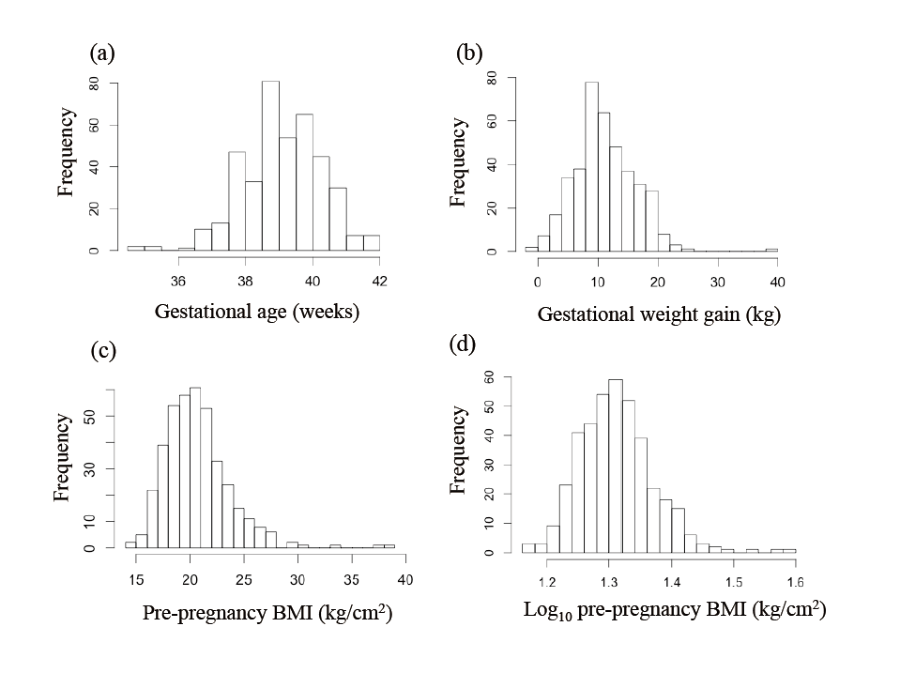
\includegraphics{Figures/Fig31.pdf}
\caption[Histograms of (a) gestational age, (b) gestational weight gain, (c) pre-pregnancy body mass index, and (d) $\log_{10}$ pre-pregnancy body mass index]{Histograms of (a) gestational age, (b) gestational weight gain, (c) prepregnancy body mass index (BMI), and (d) $\log_{10}$ pre-pregnancy BMI.}
\label{fig:Fig31}
\end{center}
\end{figure}


\begin{figure}
  \centering
  \label{fig:Fig32}
  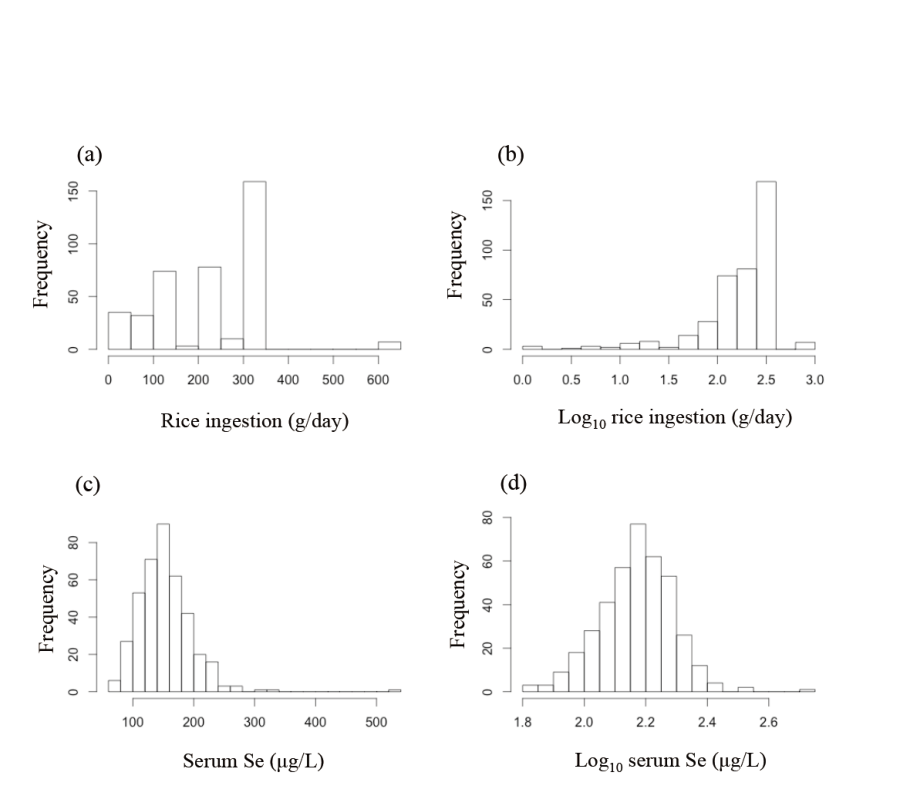
\includegraphics[scale=1]{Figures/Fig32.pdf}
  \caption[Histograms of (a) rice ingestion, (b) $\log_{10}$ rice ingestion, (c) serum selenium, and (4) $\log_{10}$ serum selenium]{Histograms of (a) rice ingestion, (b) $\log_{10}$ rice ingestion, (c) serum selenium (Se), and (4) $\log_{10}$ serum Se.}
\end{figure}

\begin{figure}
  \centering
    \label{fig:Fig33}
  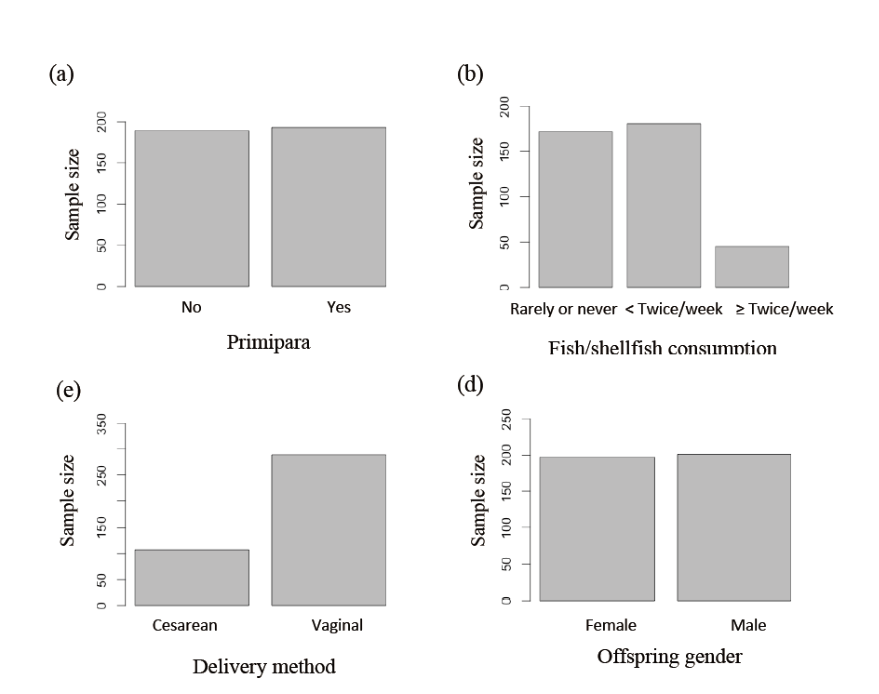
\includegraphics[scale=1]{Figures/Fig33.pdf}
  \caption[Distributions of (a) primipara, (b) fish/shellfish consumption, (c) delivery method, and (d) offspring gender]{Distributions of (a) primipara, (b) fish/shellfish consumption, (c) delivery method, and (d) offspring gender.}
\end{figure}

\begin{figure}
  \centering
    \label{fig:Fig34}
  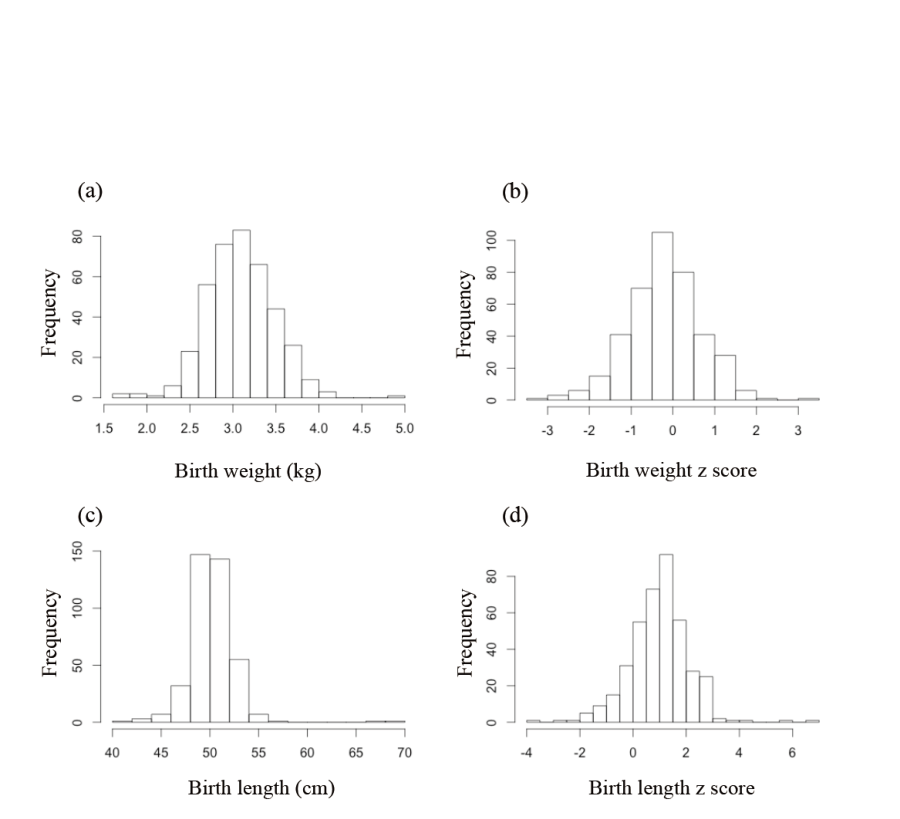
\includegraphics[scale=1]{Figures/Fig34.pdf}
  \caption[Histograms of (a) birth weight, (b) birth weight z score, (c) birth length, and (d) birth length z score]{Histograms of (a) birth weight, (b) birth weight z score, (c) birth length, and (d) birth length z score.}
\end{figure}

\begin{figure}
  \centering
    \label{fig:Fig35}
  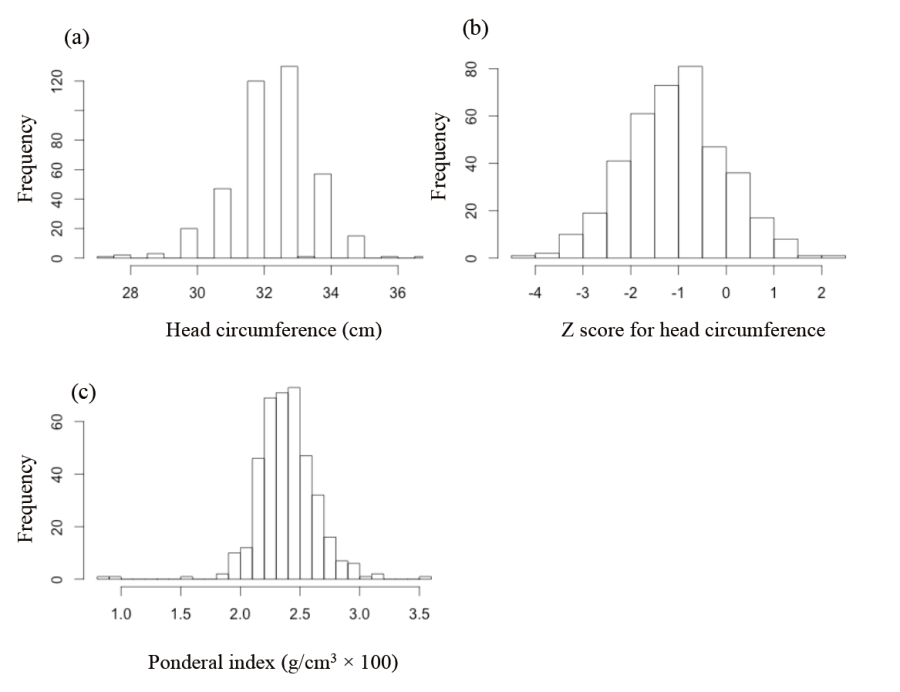
\includegraphics[scale=1]{Figures/Fig35.pdf}
  \caption[Histograms of (a) head circumference, (b) head circumference z score, and (c) ponderal index]{Histograms of (a) head circumference, (b) head circumference z score, and (c) ponderal index.}
\end{figure}

\begin{figure}
  \centering
    \label{fig:Fig36}
  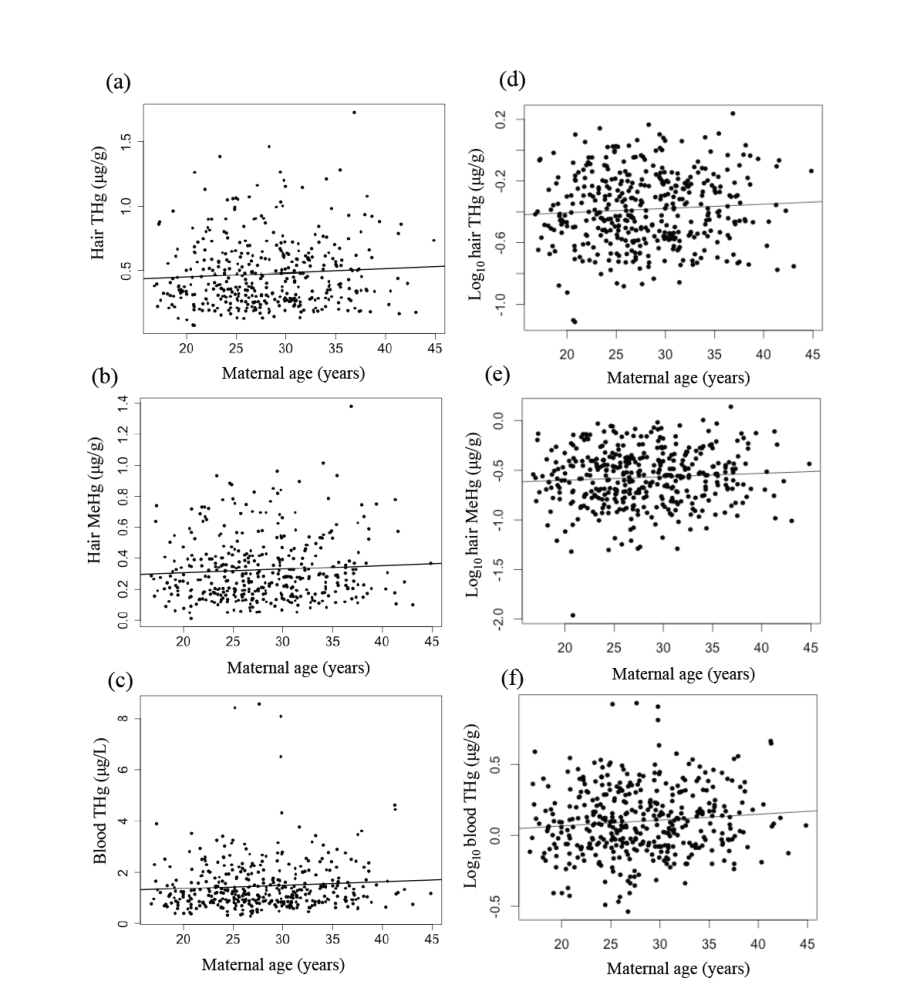
\includegraphics[scale=1]{Figures/Fig36.pdf}
  \caption[Bivariate analyses of maternal age versus mercury biomarkers]{Bivariate analyses of maternal age versus mercury biomarkers. Spearman's correlation test of maternal age versus (a) hair total mercury (THg) (rho=0.048, p=0.34), (b) hair methylmercury (MeHg) (rho=0.05, p=0.32), (c) blood THg (rho=0.087, p=0.08), and Pearson's correlation test of maternal age versus (d) $\log_{10}$ hair THg (rho=0.068, p=0.18), (e) $\log_{10}$ hair MeHg (rho=0.071, p=0.16), and (f) $\log_{10}$ blood THg (rho=0.099, p=0.06) (n=397-398 for all).}
\end{figure}

\begin{figure}
  \centering
    \label{fig:Fig37}
  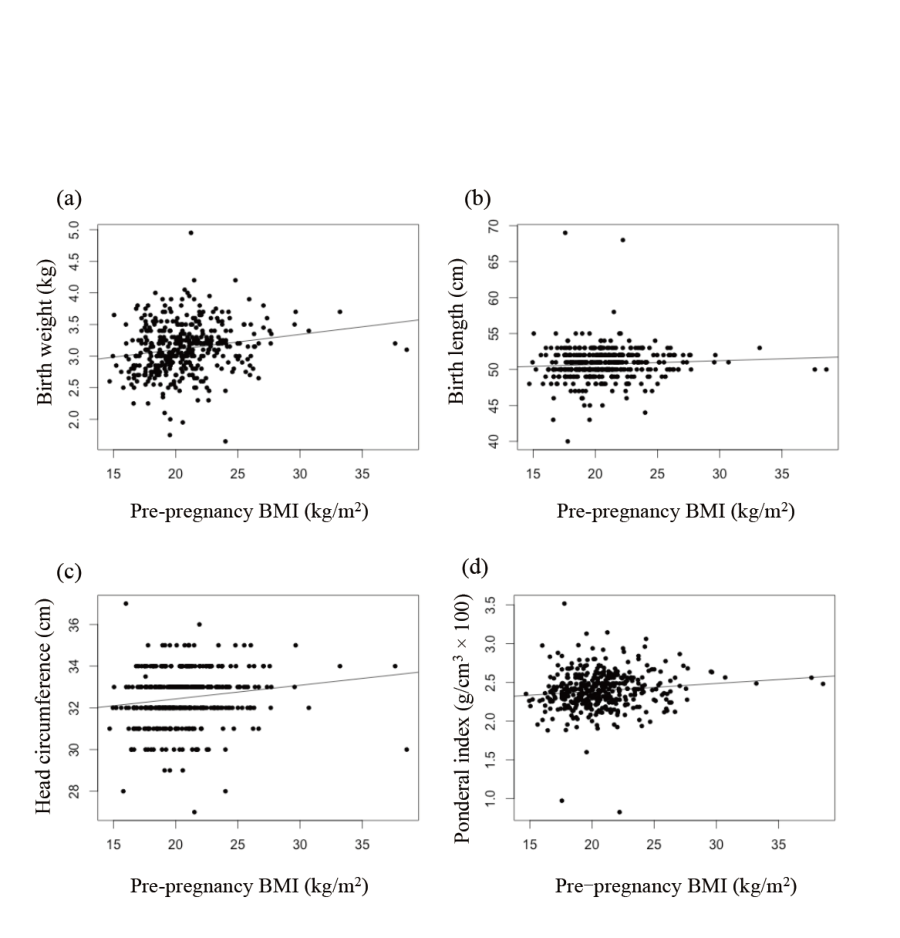
\includegraphics[scale=1]{Figures/Fig37.pdf}
  \caption[Bivariate analyses of pre-pregnancy body mass index versus birth outcomes]{Bivariate analyses of pre-pregnancy body mass index (BMI) versus birth outcomes. Spearman's correlation test of pre-pregnancy BMI versus (a) birth weight (rho = 0.21, p < 0.01), (b) birth length (rho = 0.12, p = 0.02), (c) head circumference (rho = 0.20, p < 0.01), and (d) ponderal index (rho = 0.14, p < 0.01) (Spearman's correlation test for all, n=397 for all).}
\end{figure}

\begin{figure}
  \centering
    \label{fig:Fig38}
  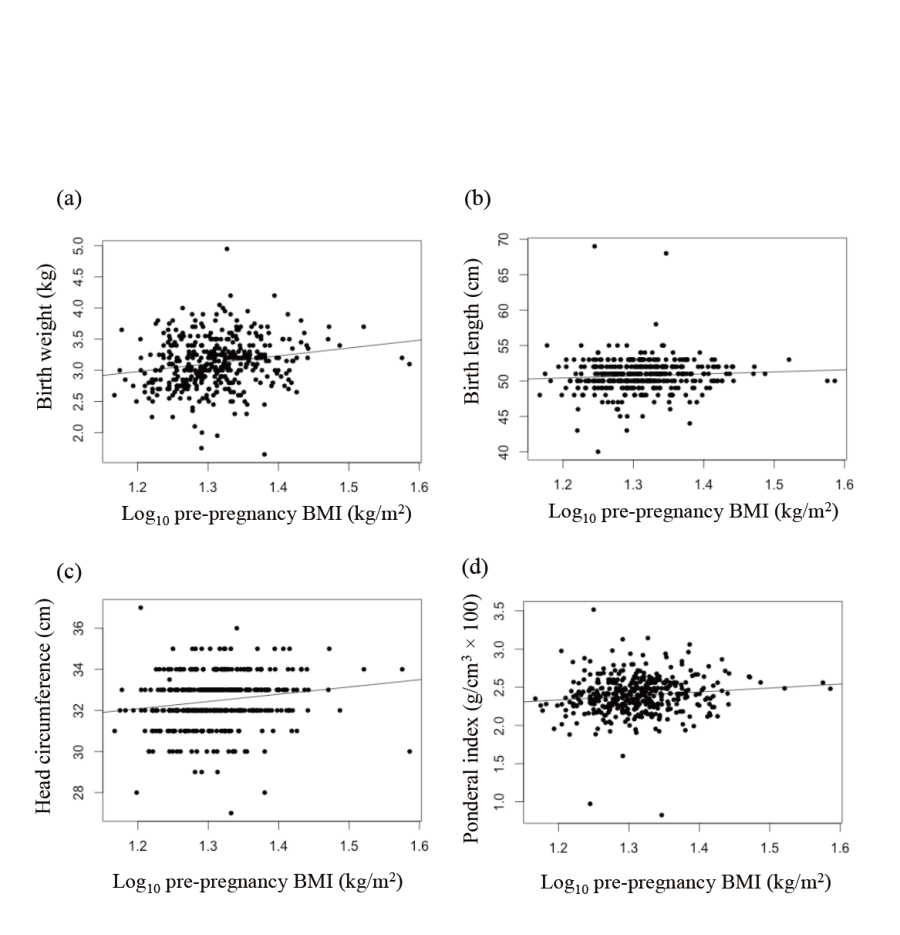
\includegraphics[scale=1]{Figures/Fig38.pdf}
  \caption[Bivariate analyses of $\log_{10}$  pre-pregnancy body mass index versus birth outcomes (birth weight, birth length, head circumference, ponderal index)]{Bivariate analyses of $\log_{10}$  pre-pregnancy body mass index (BMI) versus birth outcomes (birth weight, birth length, head circumference, ponderal index). Pearson's correlation test of $\log_{10}$  pre-pregnancy BMI versus (a) birth weight (rho = 0.19, p < 0.001), (b) birth length (rho = 0.073, p = 0.05), (c) head circumference (rho = 0.17, p < 0.001), and (d) ponderal index (rho = 0.12, p = 0.01) (Pearson's correlation test for all, n=397 for all).}
\end{figure}

\begin{figure}
  \centering
    \label{fig:Fig39}
  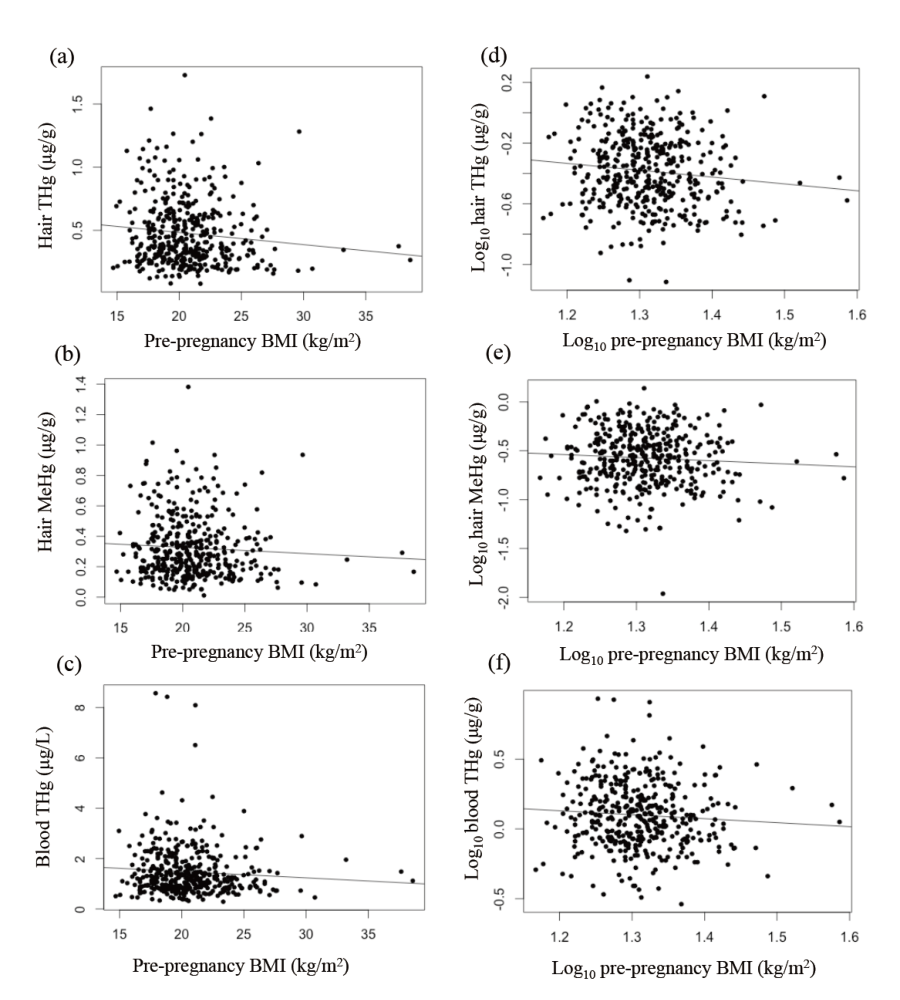
\includegraphics[scale=1]{Figures/Fig39.pdf}
  \caption[Bivariate analyses of pre-pregnancy body mass index versus mercury biomarkers]{Bivariate analyses of pre-pregnancy body mass index (BMI) versus mercury biomarkers. Spearman's correlation test of pre-pregnancy BMI versus (a) hair total mercury (THg) (rho = -0.11, p = 0.03), (b) hair methylmercury (MeHg) (rho = -0.05, p = 0.28), (c) blood THg (rho = -0.08, p = 0.09), and Pearson's correlation test of $\log_{10}$ pre-pregnancy BMI versus (a) $\log_{10}$ hair THg (rho = -0.12, p = 0.02), (b) $\log_{10}$ hair MeHg (rho = -0.07, p =0.18), (c) $\log_{10}$ blood THg (rho = -0.07, p = 0.15) (n=396-397 for all).}
\end{figure}

\begin{figure}
  \centering
    \label{fig:Fig310}
  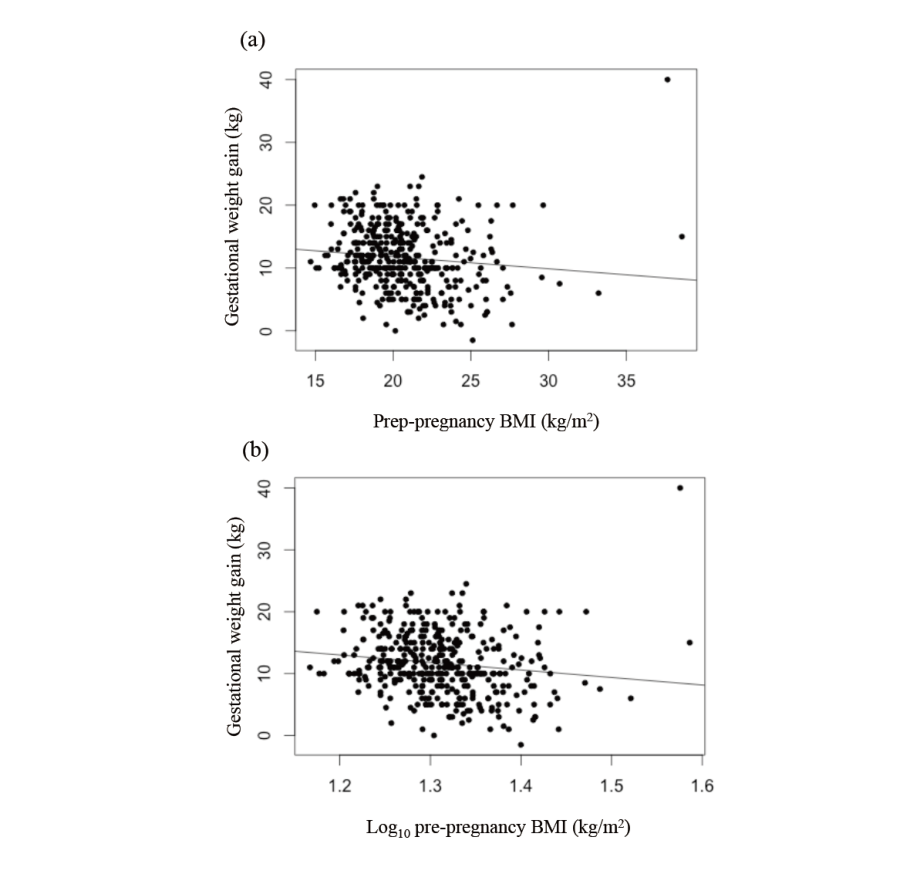
\includegraphics[scale=1]{Figures/Fig310.pdf}
  \caption[Bivariate analyses of gestational weight gain versus pre-pregnancy body mass index]{Bivariate analyses of gestational weight gain versus pre-pregnancy body mass index (BMI). (a) Gestational weight gain versus pre-pregnancy BMI (Spearman's rho = -0.23, p < 0.0001) and (b) gestational weight gain versus $\log_{10}$ pre-pregnancy BMI (Pearson's rho = -0.14, p = 0.004) (n=397 for all).}
\end{figure}

\begin{figure}
  \centering
    \label{fig:Fig311}
  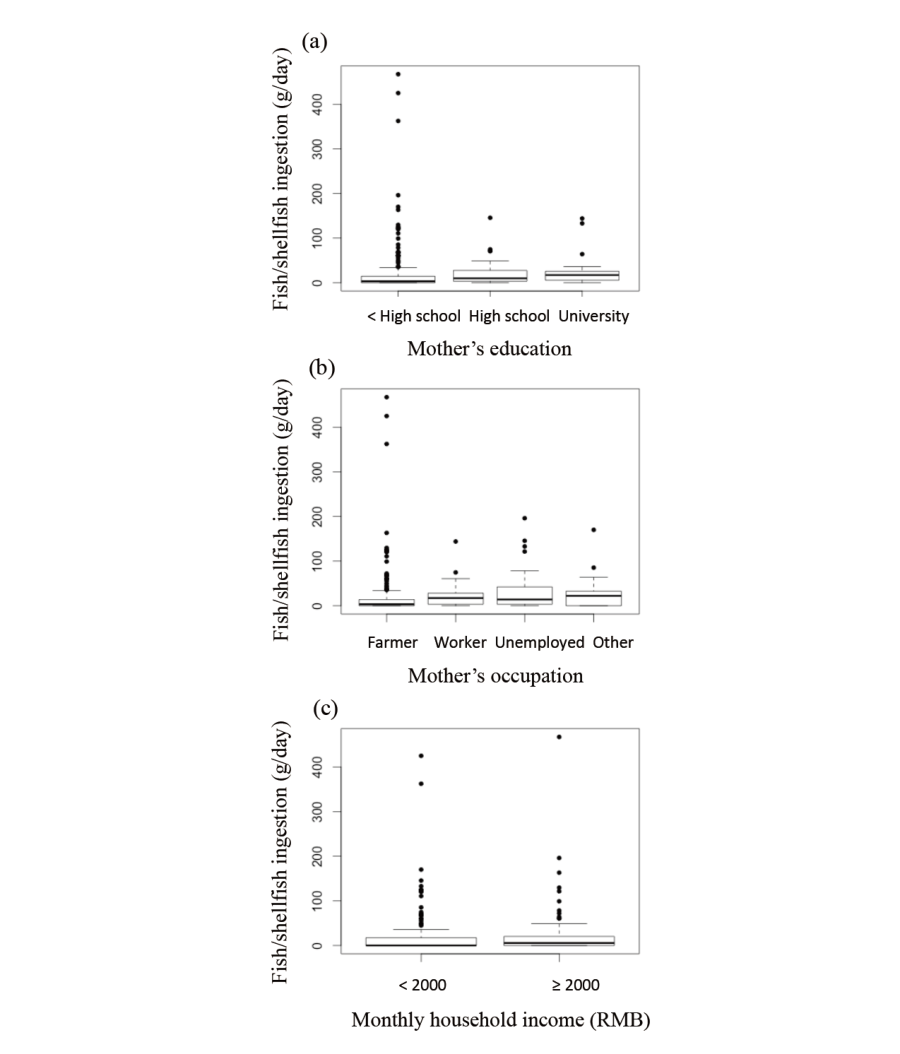
\includegraphics[scale=1]{Figures/Fig311.pdf}
  \caption[Bivariate analyses of fish/shellfish ingestion versus maternal characteristics (education, occupation, household income)]{Bivariate analyses of fish/shellfish ingestion versus maternal characteristics (education, occupation, household income). Fish/shellfish ingestion versus (a) mother's education (Kruskal-Wallis test, p < 0.01, n = 388), (b) mother's occupation (Kruskal-Wallis test, p < 0.01, n = 391), and (c) monthly household income (Wilcoxon-Mann-Whitney test, p = 0.03, n=363).}
\end{figure}

\begin{figure}
  \centering
    \label{fig:Fig312}
  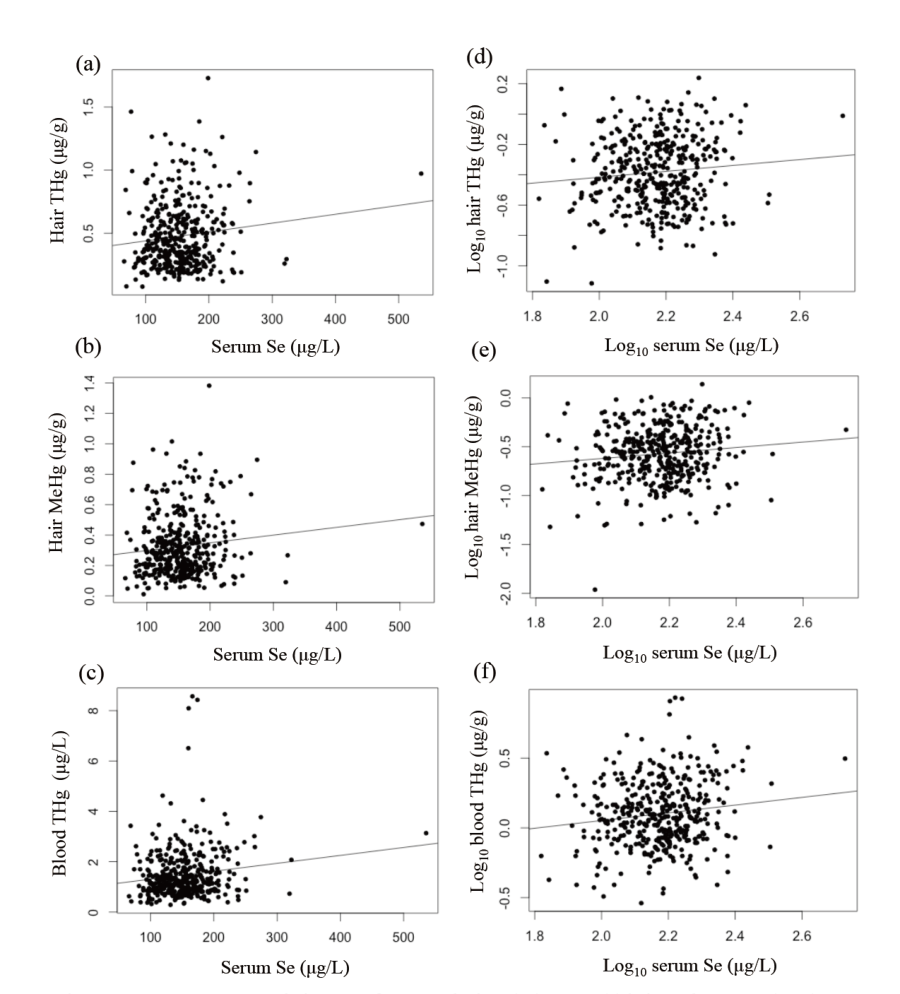
\includegraphics[scale=1]{Figures/Fig312.pdf}
  \caption[Bivariate analyses of serum selenium versus mercury biomarkers]{Bivariate analyses of serum selenium (Se) versus mercury biomarkers. Spearman's correlation test of serum Se versus (a) hair total mercury (THg) (rho = 0.06, p = 0.20), (b) hair methylmercury (MeHg) (rho = 0.09, p = 0.09), (c) blood THg (rho = 0.10, p = 0.04), and Pearson's correlation test of $\log_{10}$ serum Se versus (a) $\log_{10}$ hair THg (rho = 0.10, p = 0.08), (b) $\log_{10}$ hair MeHg (rho = 0.12, p =0.06), (c) $\log_{10}$ blood THg (rho = 0.14, p = 0.05) (n=396 for all).}
\end{figure}

\begin{figure}
  \centering
    \label{fig:Fig313}
  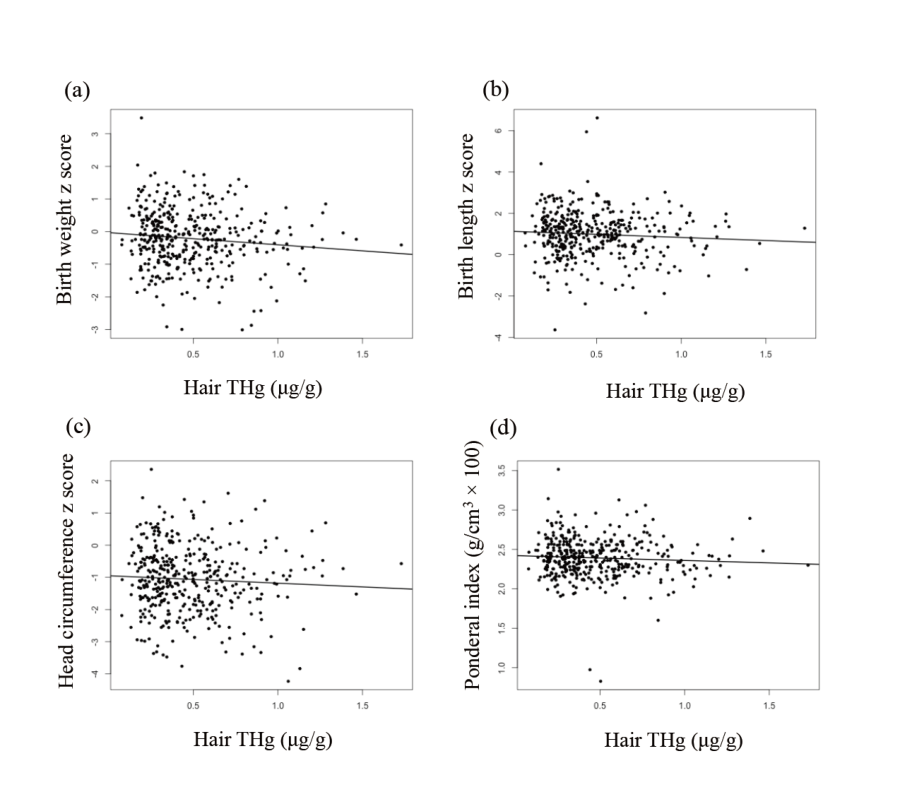
\includegraphics[scale=1]{Figures/Fig313.pdf}
  \caption[Bivariate analyses of hair total mercury versus birth outcomes (birth weight z score, birth length z score, head circumference z score, ponderal index)]{Bivariate analyses of hair total mercury (THg) versus birth outcomes (birth weight z score, birth length z score, head circumference z score, ponderal index). Spearman's correlation test of hair THg versus (a) birth weight z score (rho = -0.11, p = 0.04), (b) birth length z score (rho = -0.07, p = 0.19), (c) head circumference z score (rho = -0.07, p = 0.15), and (d) ponderal index (rho = -0.07, p = 0.15) (n=398 for all).}
\end{figure}


\begin{figure}
  \centering
    \label{fig:Fig314}
  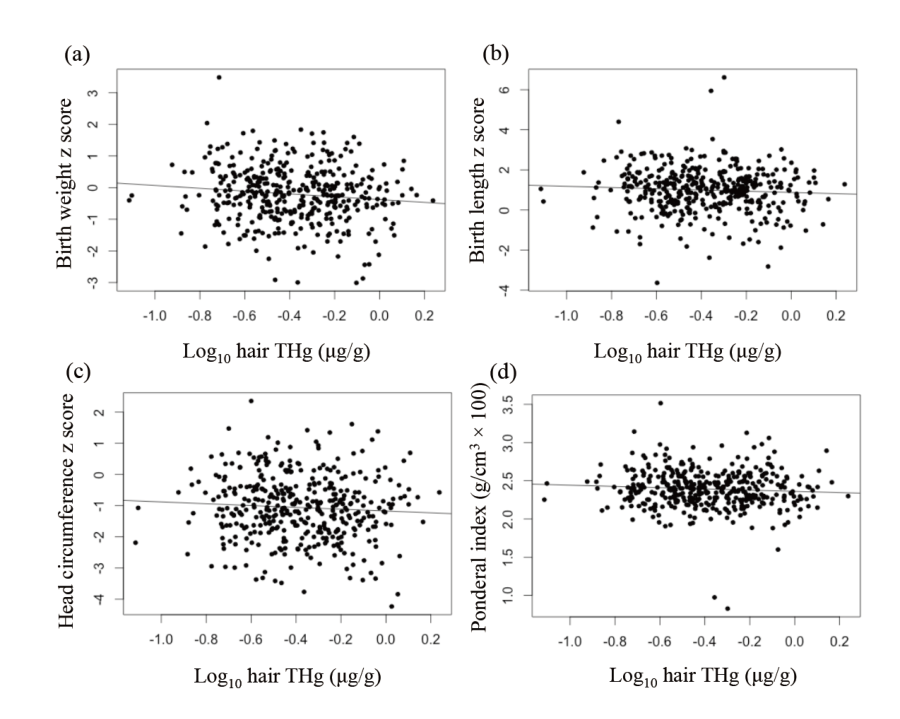
\includegraphics[scale=1]{Figures/Fig314.pdf}
  \caption[Bivariate analyses of $\log_{10}$ hair total mercury versus birth outcomes (birth weight z score, birth length z score, head circumference z score, ponderal index)]{Bivariate analyses of $\log_{10}$ hair total mercury (THg) versus birth outcomes (birth weight z score, birth length z score, head circumference z score, ponderal index). Pearson's correlation test of $\log_{10}$ hair THg versus (a) birth weight z score (rho = -0.12, p = 0.02), (b) birth length z score (rho = -0.07, p = 0.19), (c) head circumference z score (rho = -0.07, p = 0.19), and (d) ponderal index (rho = -0.08, p = 0.13) (n=398 for all).}
\end{figure}


\begin{figure}
  \centering
    \label{fig:Fig315}
  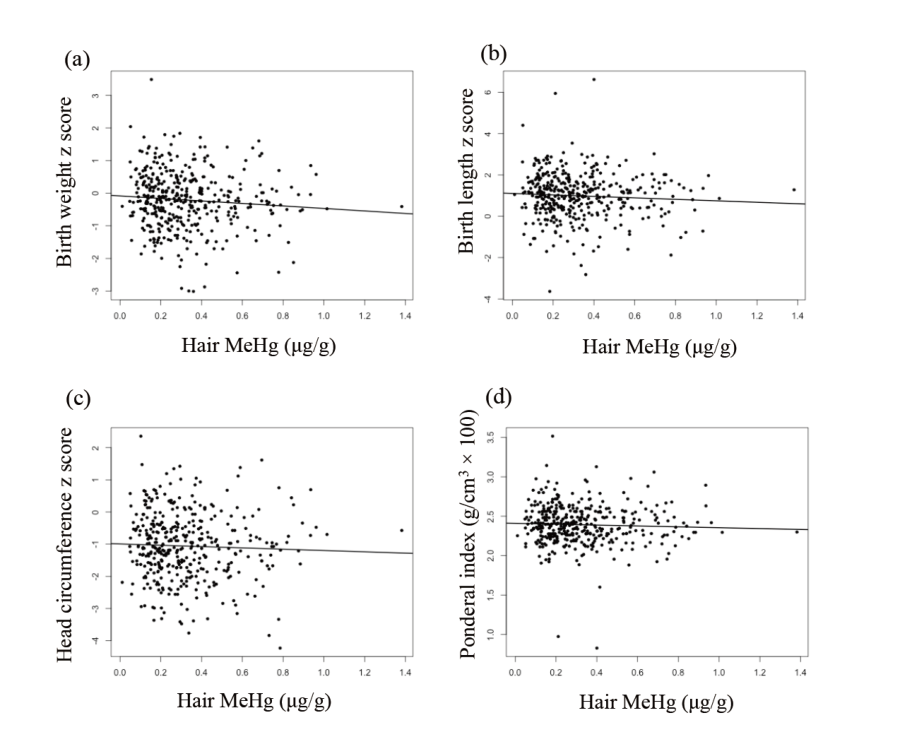
\includegraphics[scale=1]{Figures/Fig315.pdf}
  \caption[Bivariate analyses of hair methylmercury versus birth outcomes (birth weight z score, birth length z score, head circumference z score, ponderal index)]{Bivariate analyses of hair methylmercury (MeHg) versus birth outcomes (birth weight z score, birth length z score, head circumference z score, ponderal index). Spearman's correlation test of hair MeHg versus (a) birth weight z score (rho = -0.10, p = 0.05), (b) birth length z score (rho = -0.07, p = 0.16), (c) head circumference z score (rho = -0.07, p = 0.19), and (d) ponderal index (rho = -0.07, p=0.19) (n=398 for all).}
\end{figure}


\begin{figure}
  \centering
    \label{fig:Fig316}
  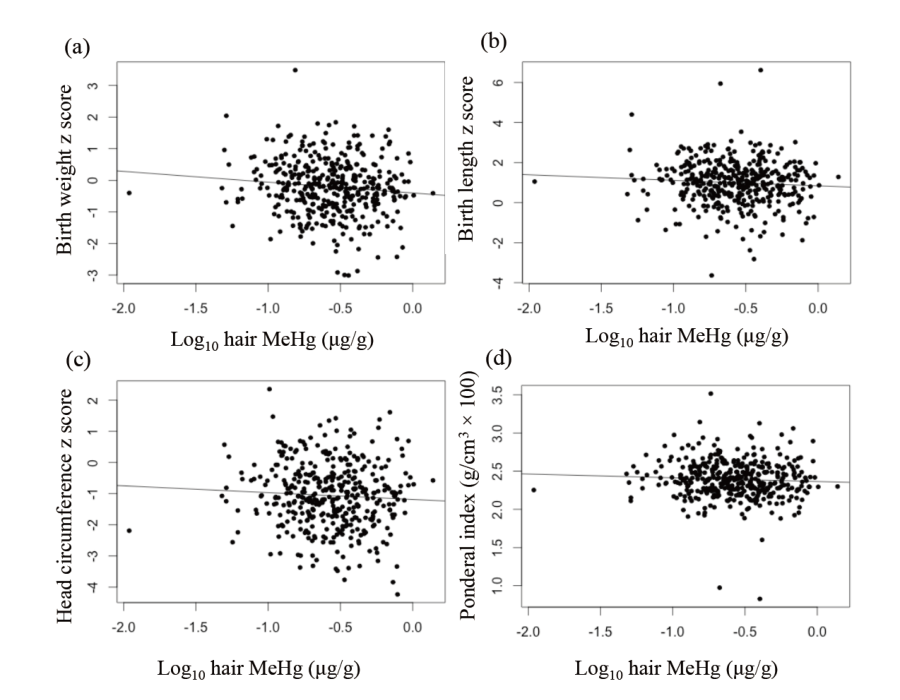
\includegraphics[scale=1]{Figures/Fig316.pdf}
  \caption[Bivariate analyses of $\log_{10}$ hair methylmercury versus birth outcomes (birth weight z score, birth length z score, head circumference z score, ponderal index)]{Bivariate analyses of $\log_{10}$ hair methylmercury (MeHg) versus birth outcomes (birth weight z score, birth length z score, head circumference z score, ponderal index). Pearson's correlation test of $\log_{10}$ hair MeHg versus (a) birth weight z score (rho = -0.11, p = 0.03), (b) birth length z score (rho = -0.07, p = 0.16), (c) head circumference z score (rho = -0.06, p = 0.24), and (d) ponderal index (rho = -0.06, p=0.27) (n=398 for
all).}
\end{figure}

\begin{figure}
  \centering
    \label{fig:Fig317}
  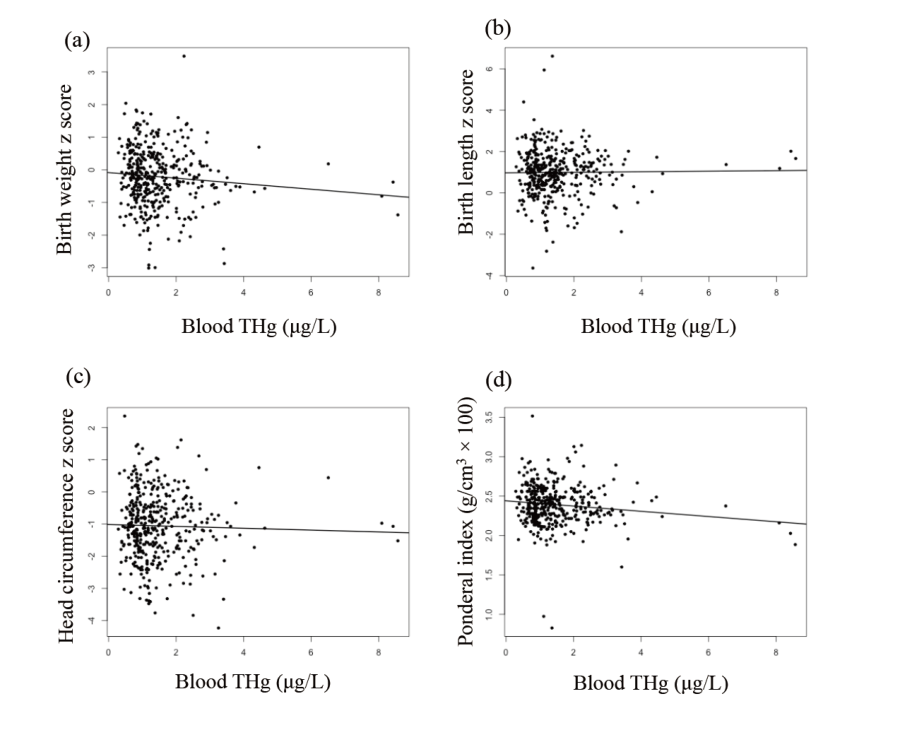
\includegraphics[scale=1]{Figures/Fig317.pdf}
  \caption[Bivariate analyses of blood total mercury versus birth outcomes (birth weight z score, birth length z score, head circumference z score, ponderal index)]{Bivariate analyses of blood total mercury (THg) versus birth outcomes (birth weight z score, birth length z score, head circumference z score, ponderal index). Spearman's correlation test of blood THg versus (a) birth weight z score (rho = -0.10, p = 0.05), (b) birth length z score (rho = 0.0014, p=0.98), (c) head circumference z score (rho = -0.03, p=0.54), and (d) ponderal index (rho = -0.11, p = 0.03) (n=397 for all).}
\end{figure}


\begin{figure}
  \centering
    \label{fig:Fig318}
  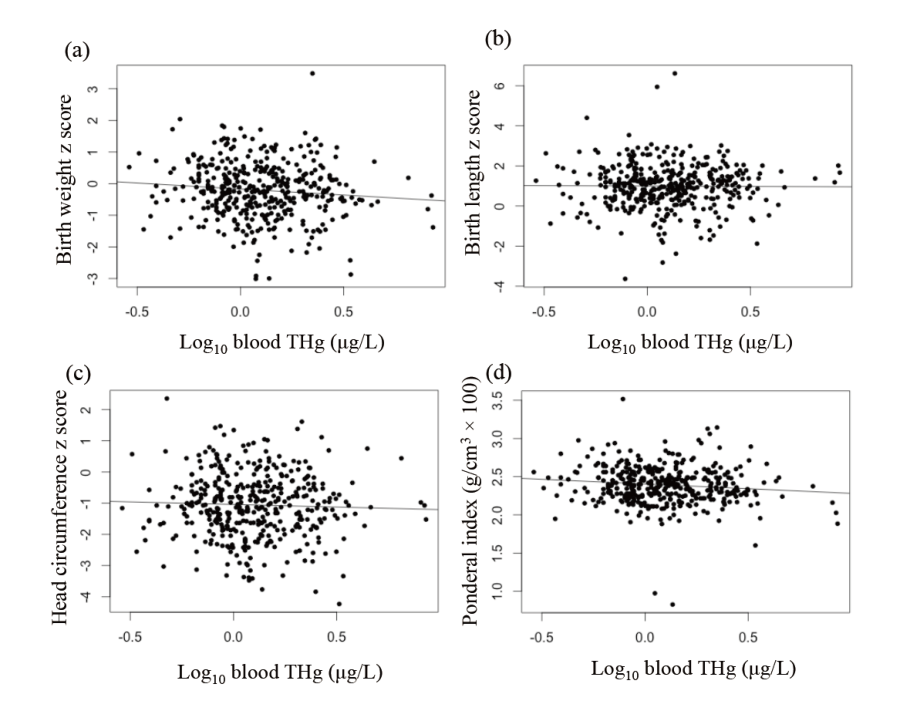
\includegraphics[scale=1]{Figures/Fig318.pdf}
  \caption[Bivariate analyses of $\log_{10}$ blood total mercury versus birth outcomes (birth weight z score, birth length z score, head circumference z score, ponderal index)]{Bivariate analyses of $\log_{10}$ blood total mercury (THg) versus birth outcomes (birth weight z score, birth length z score, head circumference z score, ponderal index). Pearson's correlation test of $\log_{10}$ blood THg versus (a) birth weight z score (rho = -0.10, p = 0.04), (b) birth length z score (rho = 0.0092, p=0.85), (c) head circumference z score (rho = -0.04, p=0.45), and (d) ponderal index (rho = -0.12, p = 0.02) (n=397 for all).}
\end{figure}


%\begin{figure}
%  \centering
%    \label{fig:Fig319}
%  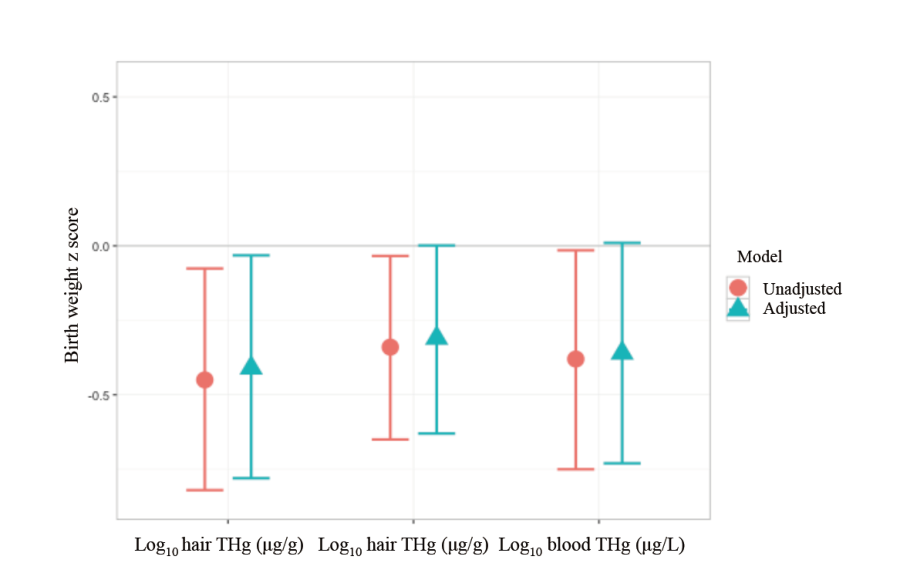
\includegraphics[scale=1]{Figures/Fig319.pdf}
%  \caption[Betas and 95\% confidence intervals for birth weight z score related to $\log_{10}$ hair total mercury, $\log_{10}$ hair methylmercury, and $\log_{10}$ blood total mercury in unadjusted and adjusted models]{Betas and 95\% confidence intervals (CIs) for birth weight z score related to $\log_{10}$ hair total mercury (THg), $\log_{10}$ hair methylmercury (MeHg), and $\log_{10}$ blood THg in unadjusted and adjusted models.}
%\end{figure}
%
%
%\begin{figure}
%  \centering
%    \label{fig:Fig320}
%  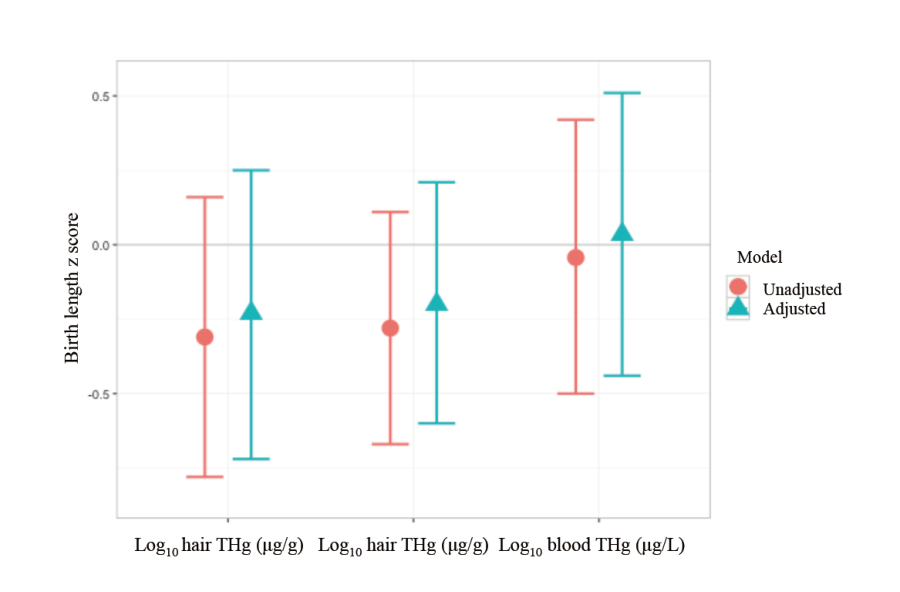
\includegraphics[scale=1]{Figures/Fig320.pdf}
%  \caption[Betas and 95\% confidence intervals for birth length z score related to $\log_{10}$ hair total mercury, $\log_{10}$ hair methylmercury, and $\log_{10}$ blood  total mercury in unadjusted and adjusted models]{Betas and 95\% confidence intervals (CIs) for birth length z score related to $\log_{10}$ hair total mercury (THg), $\log_{10}$ hair methylmercury (MeHg), and $\log_{10}$ blood THg in unadjusted and adjusted models.}
%\end{figure}
%
%
%\begin{figure}
%  \centering
%    \label{fig:Fig321}
%  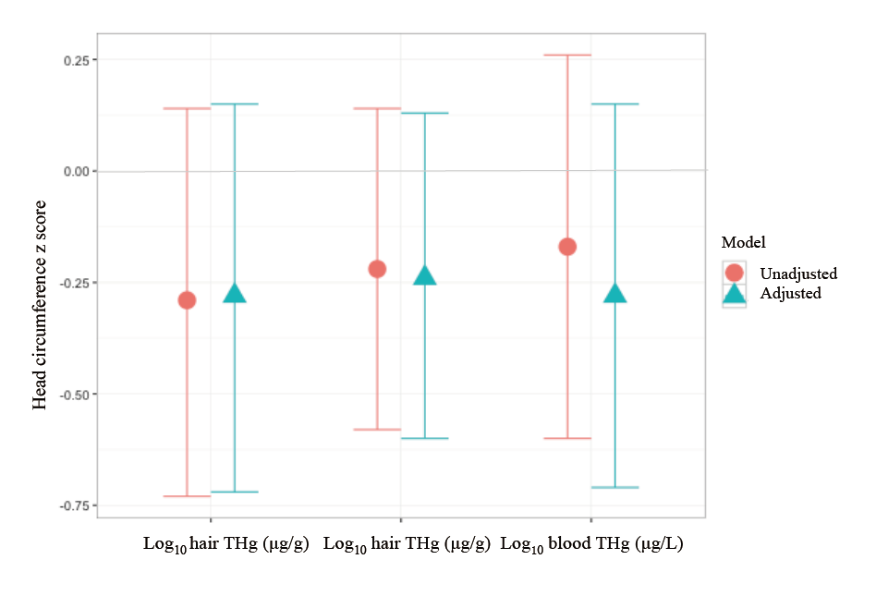
\includegraphics[scale=1]{Figures/Fig321.pdf}
%  \caption[Betas and 95\% confidence intervals for head circumference z score related to $\log_{10}$ hair total mercury, $\log_{10}$ hair methylmercury, and $\log_{10}$ blood total mercury in unadjusted and adjusted models]{Betas and 95\% confidence intervals (CIs) for head circumference z score related to $\log_{10}$ hair total mercury (THg), $\log_{10}$ hair methylmercury (MeHg), and $\log_{10}$ blood THg in unadjusted and adjusted models.}
%\end{figure}
%
%
%\begin{figure}
%  \centering
%    \label{fig:Fig322}
%  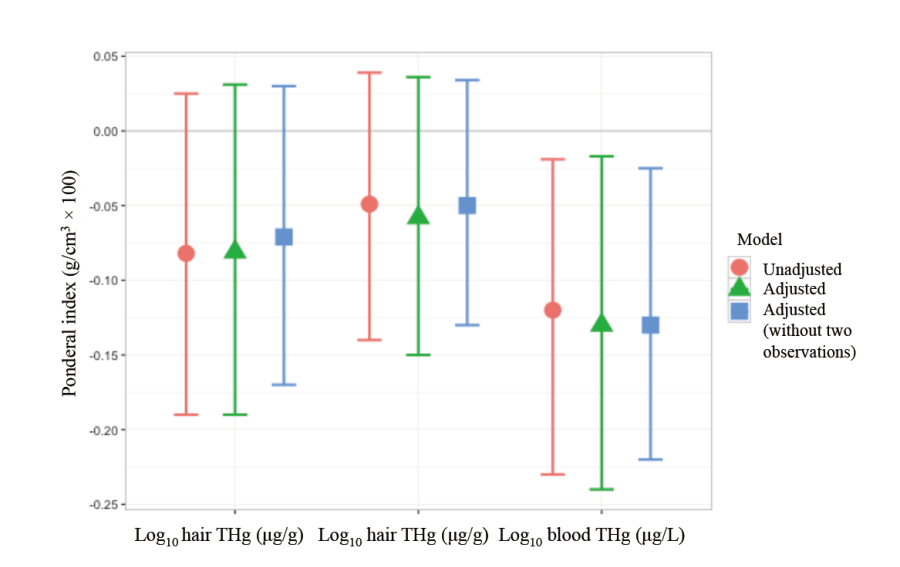
\includegraphics[scale=1]{Figures/Fig322.pdf}
%  \caption[Betas and 95\% confidence intervals for ponderal index related to $\log_{10}$ hair total mercury, $\log_{10}$ hair methylmercury, and $\log_{10}$ blood total mercury in unadjusted and adjusted models (with and without two outliers)]{Betas and 95\% confidence intervals (CIs) for ponderal index related to $\log_{10}$ hair total mercury (THg), $\log_{10}$ hair methylmercury (MeHg), and $\log_{10}$ blood THg in unadjusted and adjusted models (with and without two outliers).}
%\end{figure}
%
%
%\begin{figure}
%  \centering
%    \label{fig:Fig323}
%  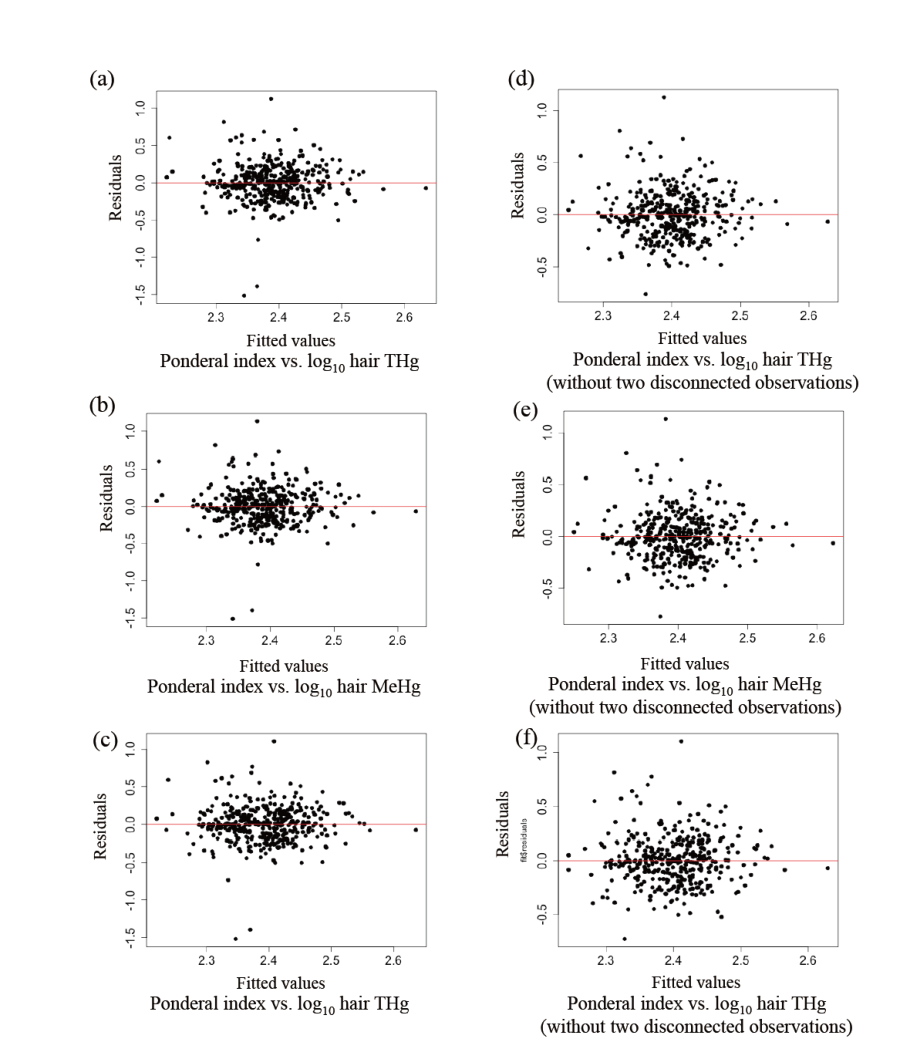
\includegraphics[scale=1]{Figures/Fig323.pdf}
%  \caption[Residuals versus fitted values plots of multiple linear regression models]{Residuals versus fitted values plots of multiple linear regression models. (a) and (d) for ponderal index versus $\log_{10}$ hair total mercury (THg), (b) and (e) for ponderal index versus $\log_{10}$ methylmercury (MeHg), (c) and (f) for ponderal index versus $\log_{10}$ blood THg. (a)-(c) for all participant, and (d)-(f) for participants without two disconnected observations.}
%\end{figure}
%
%
%\begin{figure}
%  \centering
%    \label{fig:Fig324}
%  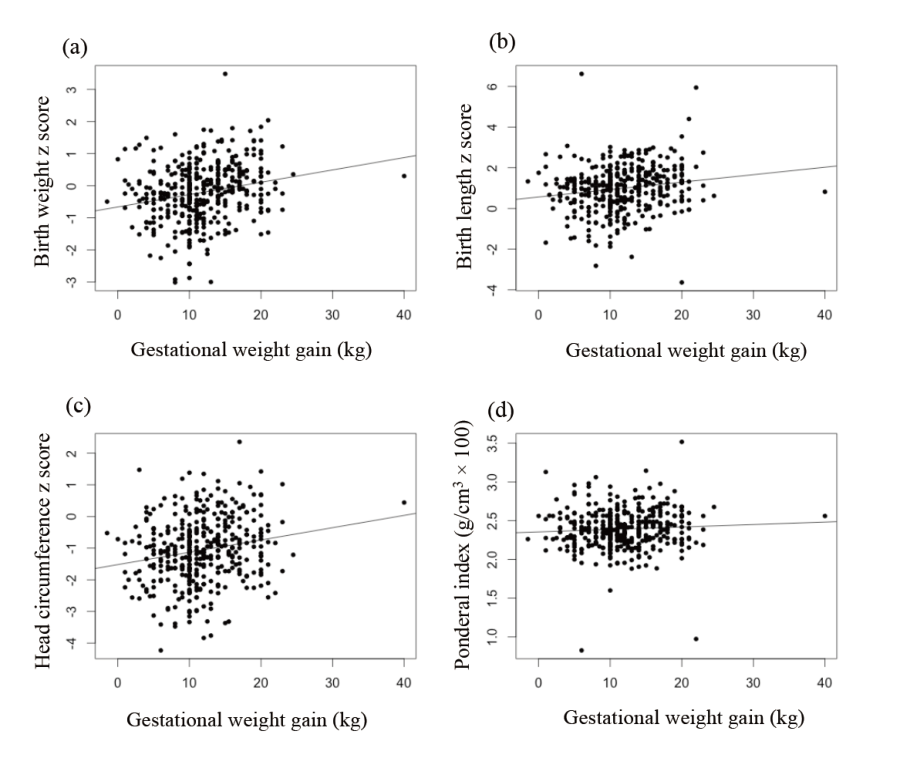
\includegraphics[scale=1]{Figures/Fig324.pdf}
%  \caption[Bivariate analyses of maternal gestational weight gain versus birth outcomes (birth weight z score, birth length z score, head circumference z score, ponderal index)]{Bivariate analyses of maternal gestational weight gain versus birth outcomes (birth weight z score, birth length z score, head circumference z score, ponderal index). Pearson's correlation test of gestational weight gain versus (a) birth weight z score (rho = 0.22, p < 0.0001), (b) birth length z score (rho = 0.17, p < 0.001), (c) head circumference z score (rho = 0.19, p < 0.001), (d) ponderal index (rho = 0.06, p = 0.20) (n=397 for all).}
%\end{figure}
%
%
%\begin{figure}
%  \centering
%    \label{fig:Fig325}
%  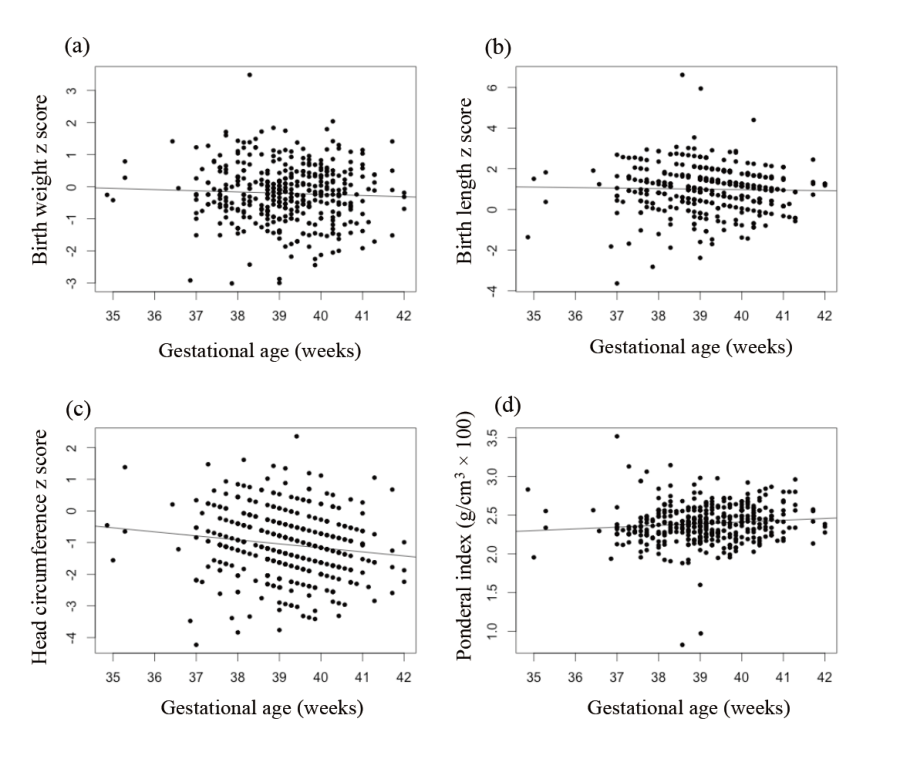
\includegraphics[scale=1]{Figures/Fig325.pdf}
%  \caption[Bivariate analyses of gestational age versus birth outcomes (birth weight z score, birth length z score, head circumference z score, ponderal index)]{Bivariate analyses of gestational age versus birth outcomes (birth weight z score, birth length z score, head circumference z score, ponderal index). Pearson's correlation test of gestational age versus (a) birth weight z score (rho = -0.05, p = 0.33), (b) birth length z score (rho = -0.03, p = 0.59), (c) head circumference z score (rho = -0.14, p = 0.004), (d) ponderal index (rho = 0.10, p = 0.04) (n=398 for all).}
%\end{figure}
%
%
%\begin{figure}
%  \centering
%    \label{fig:Fig326}
%  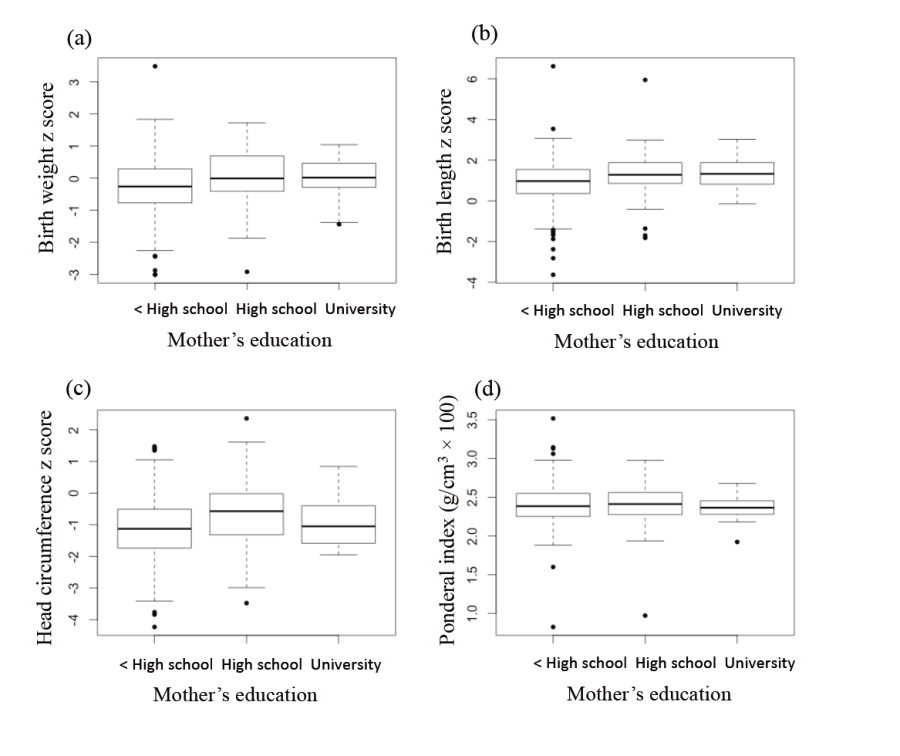
\includegraphics[scale=1]{Figures/Fig326.pdf}
%  \caption[Bivariate analyses of mother's education versus birth outcomes (birth weight z score, birth length z score, head circumference z score, ponderal index)]{Bivariate analyses of mother's education versus birth outcomes (birth weight z score, birth length z score, head circumference z score, ponderal index). One-way ANOVA test of mother's education versus (a) birth weight z score (p = 0.08), (b) birth length z score (p = 0.04), (c) head circumference z score (p = 0.02), (d) ponderal index (p = 0.90) (n=388 for all).}
%\end{figure}
%
%
%\begin{figure}
%  \centering
%    \label{fig:Fig327}
%  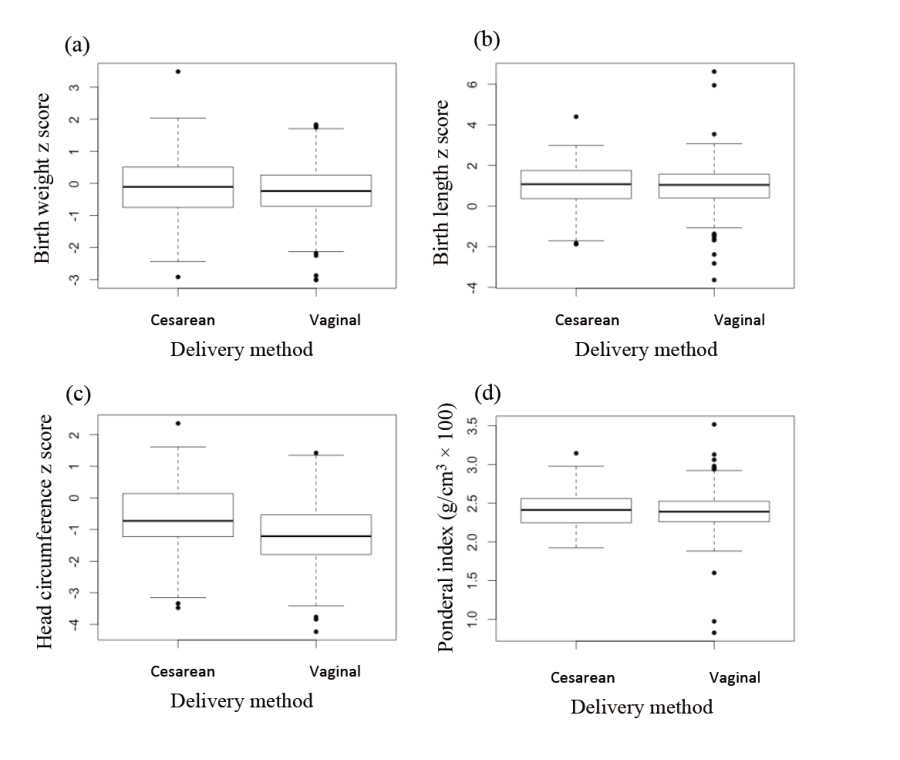
\includegraphics[scale=1]{Figures/Fig327.pdf}
%  \caption[Bivariate analyses of delivery method versus birth outcomes (birth weight z score, birth length z score, head circumference z score, ponderal index)]{Bivariate analyses of delivery method versus birth outcomes (birth weight z score, birth length z score, head circumference z score, ponderal index). Student's t-test of delivery method versus (a) birth weight z score (p = 0.17), (b) birth length z score (p = 0.59), (c) head circumference z score (p < 0.01), (d) ponderal index (p = 0.70) (n=398 for all).}
%\end{figure}
%
%\begin{figure}
%  \centering
%    \label{fig:Fig328}
%  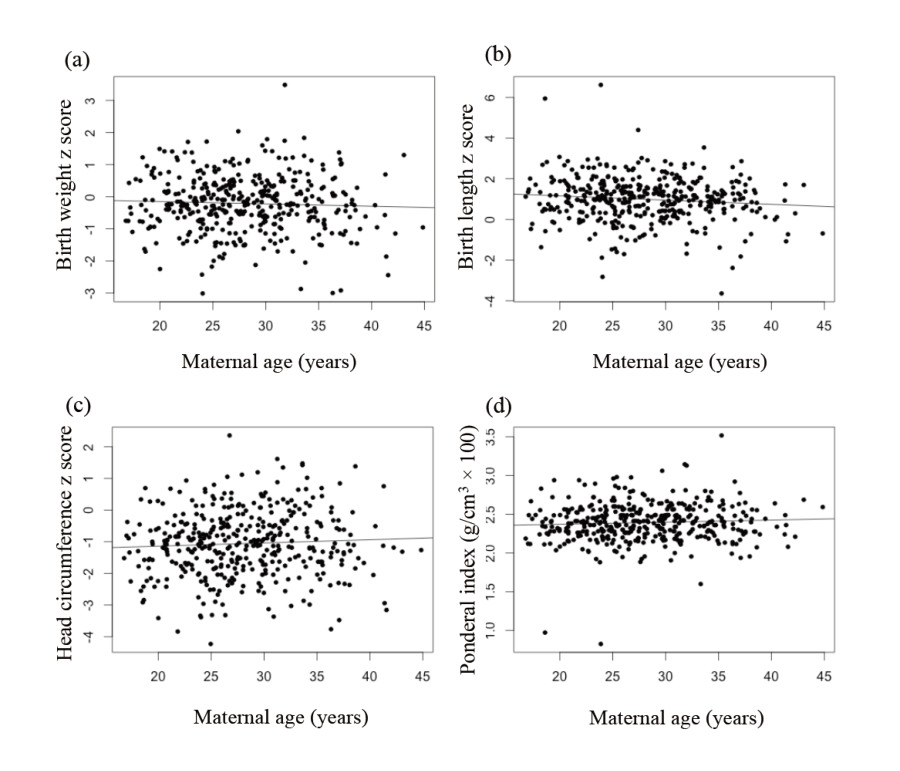
\includegraphics[scale=1]{Figures/Fig328.pdf}
%  \caption[Bivariate analyses of maternal age versus birth outcomes (birth weight z score, birth length z score, head circumference z score, ponderal index)]{Bivariate analyses of maternal age versus birth outcomes (birth weight z score, birth length z score, head circumference z score, ponderal index). Pearson's correlation test of maternal age versus (a) birth weight z score (rho = -0.05, p = 0.35), (b) birth length z score (rho = -0.11, p = 0.13), (c) head circumference z score (rho = 0.06, p=0.27), and (d) ponderal index (rho = 0.06, p = 0.22) (n=398 for all).}
%\end{figure}
%
%\begin{figure}
%  \centering
%    \label{fig:Fig329}
%  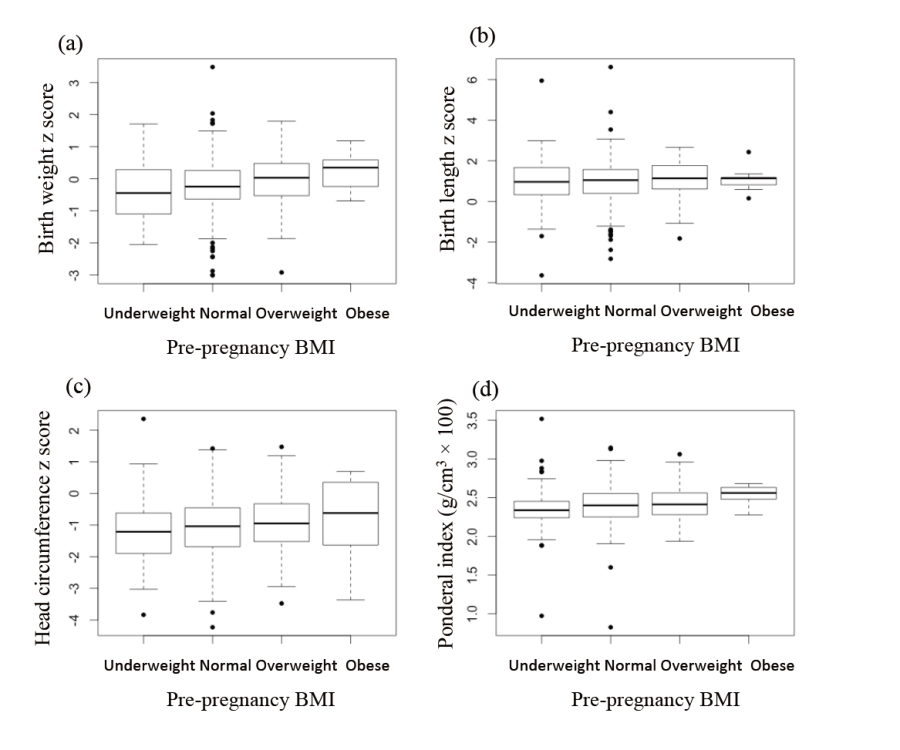
\includegraphics[scale=1]{Figures/Fig329.pdf}
%  \caption[Bivariate analyses of maternal pre-pregnancy body mass index versus birth outcomes (birth weight z score, birth length z score, head circumference z score, ponderal index)]{Bivariate analyses of maternal pre-pregnancy body mass index (BMI) versus birth outcomes (birth weight z score, birth length z score, head circumference z score, ponderal index). One-way ANOVA test of pre-pregnancy BMI versus (a) birth weight z score (p = 0.11), (b) birth length z score (p = 0.97), (c) head circumference z score (p = 0.28), (d) ponderal index (p = 0.10) (n=397 for all).}
%\end{figure}
%
%\begin{figure}
%  \centering
%    \label{fig:Fig330}
%  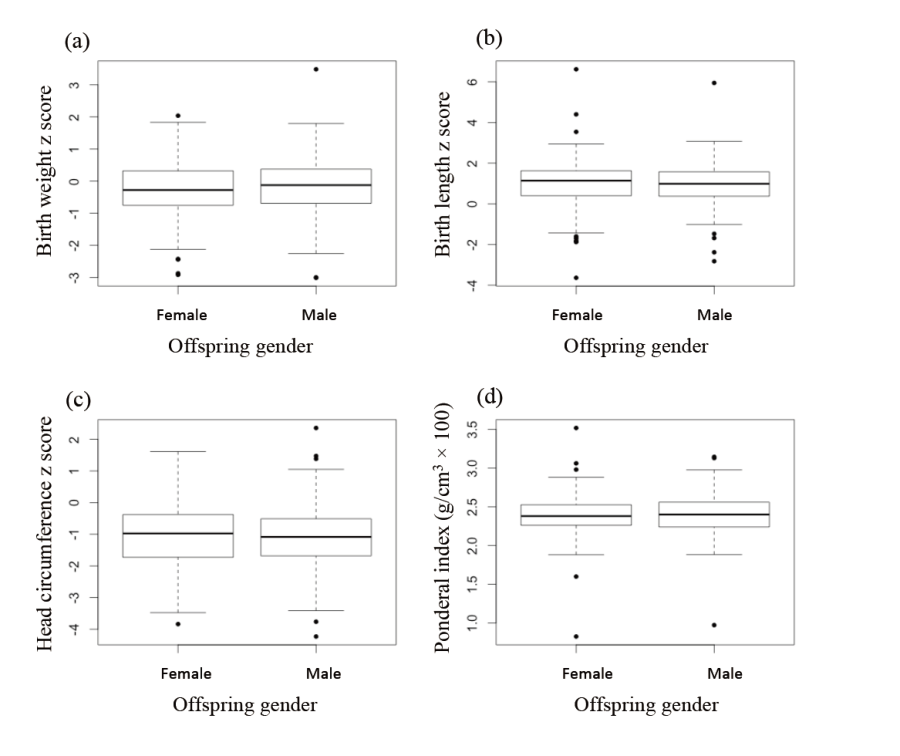
\includegraphics[scale=1]{Figures/Fig330.pdf}
%  \caption[Bivariate analyses of offspring gender versus birth outcomes (birth weight z score, birth length z score, head circumference z score, ponderal index)]{Bivariate analyses of offspring gender versus birth outcomes (birth weight z score, birth length z score, head circumference z score, ponderal index). Student's t-test of offspring gender versus (a) birth weight z score (p = 0.30), (b) birth length z score (p = 0.66), (c) head circumference z score (p = 0.65), (d) ponderal index (p = 0.60) (n=398 for all).}
%\end{figure}
%
%\begin{figure}
%  \centering
%    \label{fig:Fig331}
%  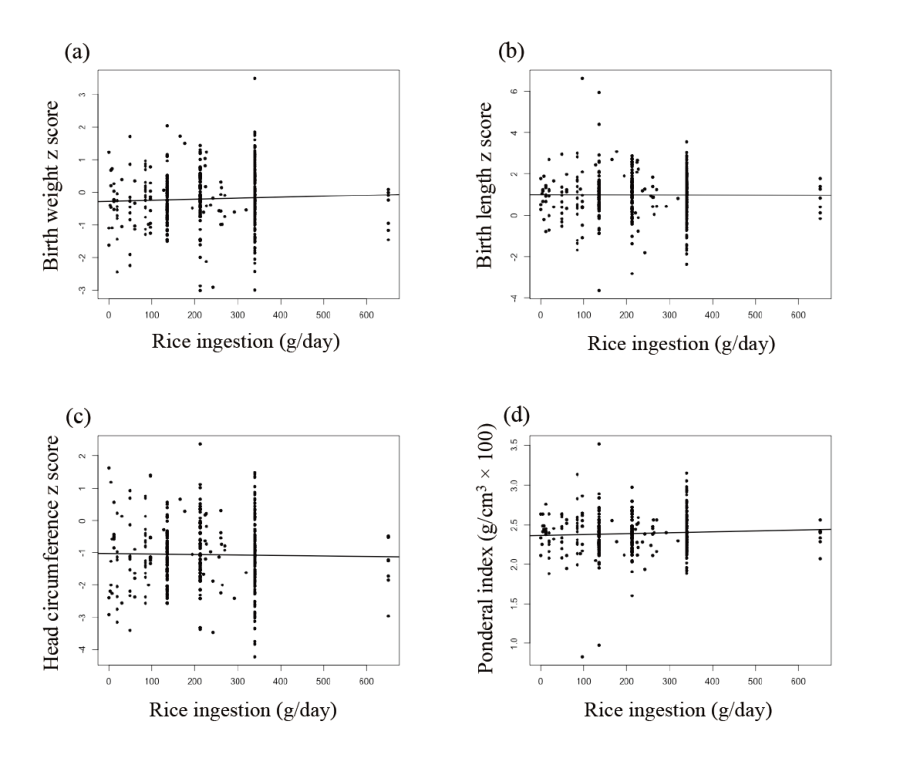
\includegraphics[scale=1]{Figures/Fig331.pdf}
%  \caption[Bivariate analyses of rice ingestion versus birth outcomes (birth weight z score, birth length z score, head circumference z score, ponderal index)]{Bivariate analyses of rice ingestion versus birth outcomes (birth weight z score, birth length z score, head circumference z score, ponderal index). Spearman's correlation test of rice ingestion versus (a) birth weight z score (rho = 0.06, p = 0.20), (b) birth length z score (rho = 0.03, p = 0.55), (c) head circumference z score (rho = 0.01, p = 0.82), (d) ponderal index (rho = 0.04, p = 0.41) (n=398 for all).}
%\end{figure}
%
%\begin{figure}
%  \centering
%    \label{fig:Fig332}
%  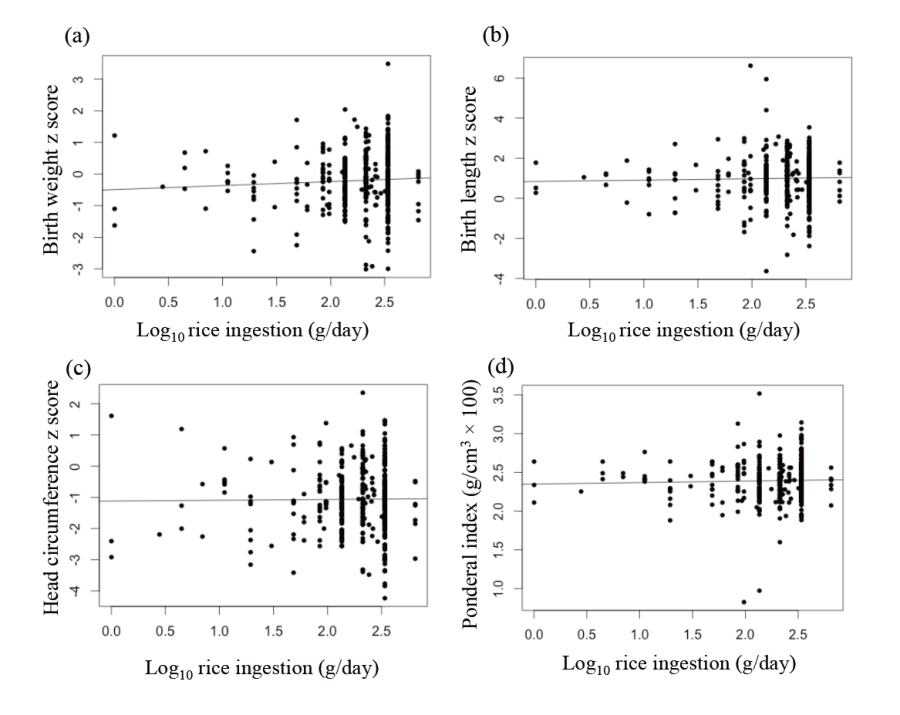
\includegraphics[scale=1]{Figures/Fig332.pdf}
%  \caption[Bivariate analyses of $\log_{10}$ rice ingestion versus birth outcomes (birth weight z score, birth length z score, head circumference z score, ponderal index)]{Bivariate analyses of $\log_{10}$ rice ingestion versus birth outcomes (birth weight z score, birth length z score, head circumference z score, ponderal index). Pearson's correlation test of $\log_{10}$ rice ingestion versus (a) birth weight z score (rho = 0.06, p = 0.23), (b) birth length z score (rho = 0.03, p = 0.61), (c) head circumference z score (rho = 0.01, p = 0.84), (d) ponderal index (rho = 0.03, p = 0.52) (n=398 for all).}
%\end{figure}
%
%\begin{figure}
%  \centering
%    \label{fig:Fig333}
%  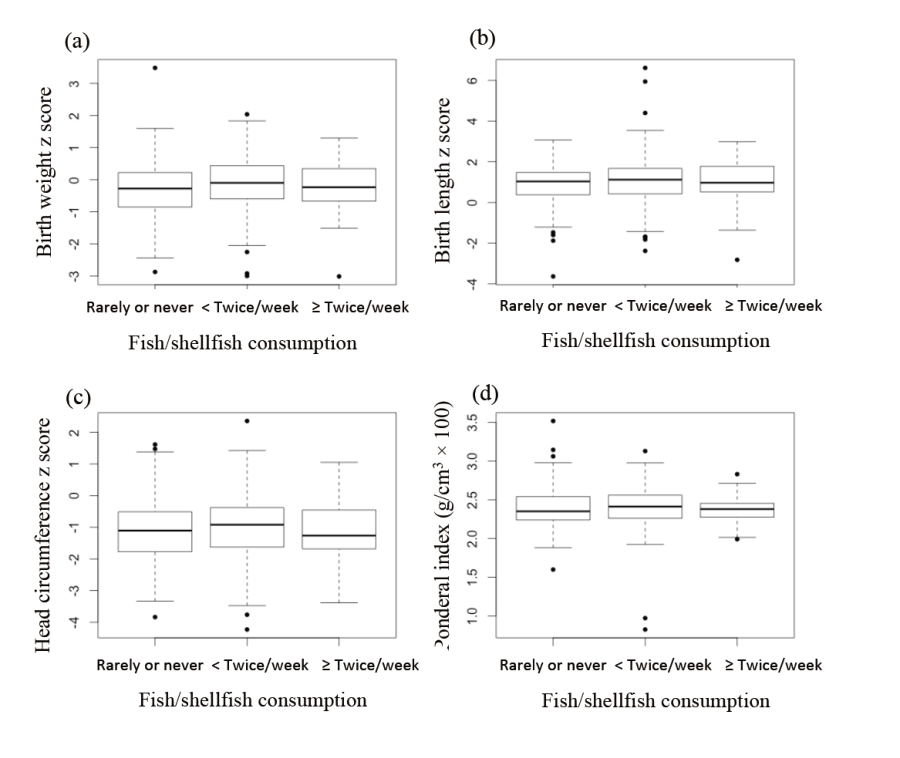
\includegraphics[scale=1]{Figures/Fig333.pdf}
%  \caption[Bivariate analyses of fish/shellfish consumption versus birth outcomes (birth weight z score, birth length z score, head circumference z score, ponderal index)]{Bivariate analyses of fish/shellfish consumption versus birth outcomes (birth weight z score, birth length z score, head circumference z score, ponderal index). Oneway ANOVA test of fish/shellfish consumption versus (a) birth weight z score (p = 0.15), (b) birth length z score (p = 0.52), (c) head circumference z score (p = 0.48), and (d) ponderal index (p = 0.82) (n=398 for all).}
%\end{figure}
%
%\begin{figure}
%  \centering
%    \label{fig:Fig334}
%  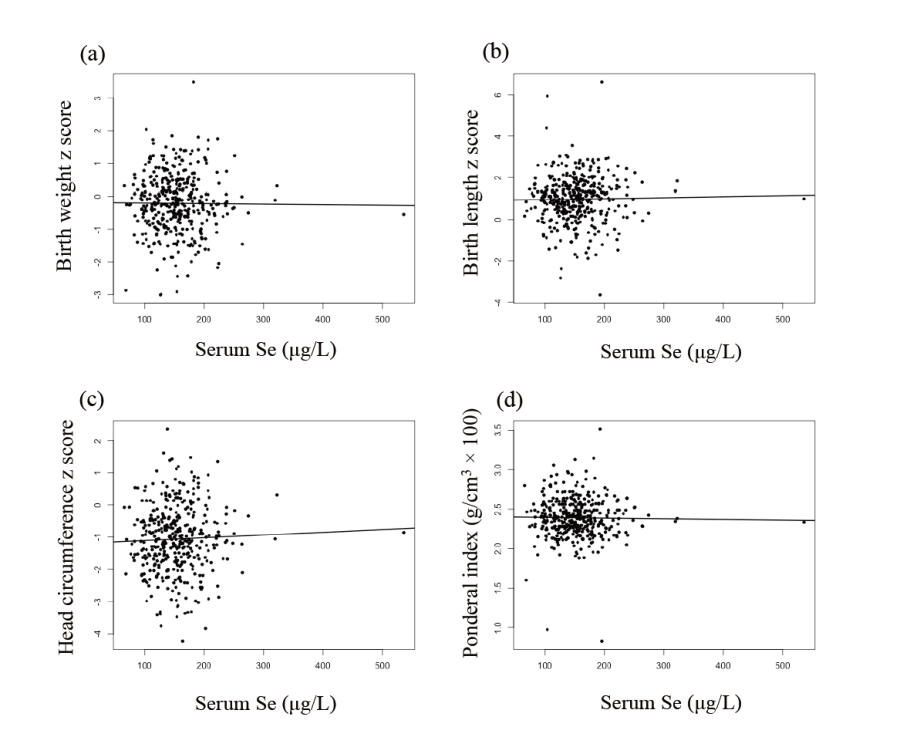
\includegraphics[scale=1]{Figures/Fig334.pdf}
%  \caption[Bivariate analyses of serum selenium versus birth outcomes (birth weight z score, birth length z score, head circumference z score, ponderal index)]{Bivariate analyses of serum selenium (Se) versus birth outcomes (birth weight z score, birth length z score, head circumference z score, ponderal index). Spearman's correlation test of serum Se versus (a) birth weight z score (rho = -0.03, p = 0.60), (b) birth length z score (rho = 0.06, p = 0.28), (c) head circumference z score (rho = 0.04, p = 0.47), and (d) ponderal index (rho = -0.03, p = 0.59) (n=396 for all).}
%\end{figure}
%
%\begin{figure}
%  \centering
%    \label{fig:Fig335}
%  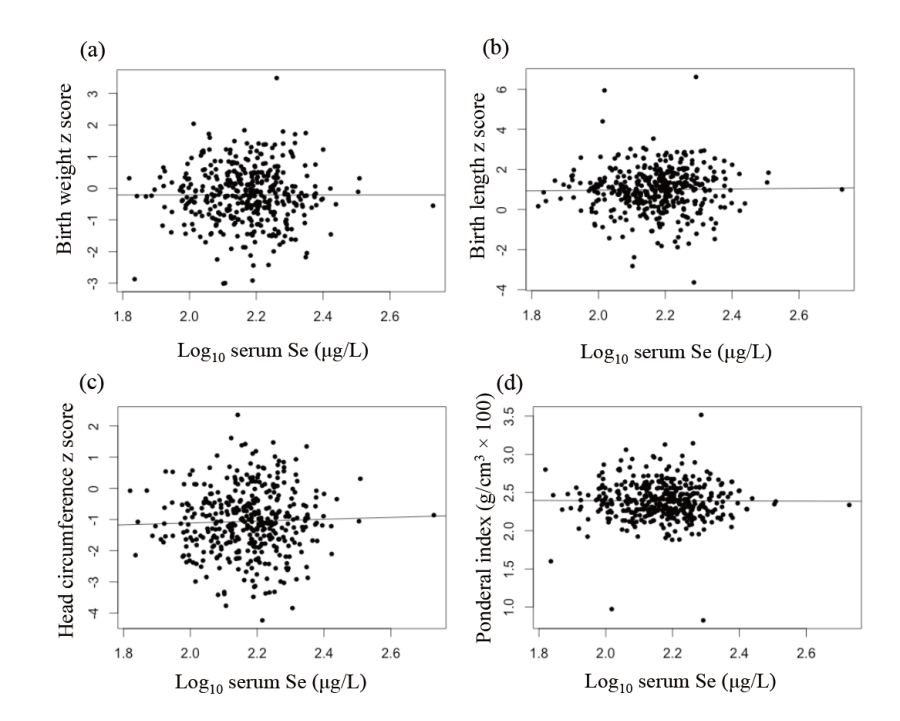
\includegraphics[scale=1]{Figures/Fig335.pdf}
%  \caption[Bivariate analyses of $\log_{10}$ serum selenium versus birth outcomes (birth weight z score, birth length z score, head circumference z score, ponderal index)]{Bivariate analyses of $\log_{10}$ serum selenium (Se) versus birth outcomes (birth weight z score, birth length z score, head circumference z score, ponderal index). Pearson's correlation test of $\log_{10}$ serum Se versus (a) birth weight z score (rho = -0.00001, p = 1.0), (b) birth length z score (rho = 0.02, p = 0.74), (c) head circumference z score (rho = 0.03, p = 0.50), and (d) ponderal index (rho = -0.0053, p = 0.92) (n=396 for all).}
%\end{figure}

